\documentclass[chaparabic,ceng,ms,12pt,oneandhalf]{metu}
\usepackage{appendix}
\usepackage{longtable}
\usepackage[pdftex]{hyperref}
\usepackage[all]{hypcap}
\usepackage{todonotes}
\usepackage{graphicx}
\graphicspath{ {./images/} }
\usepackage[figuresright]{rotating}
\usepackage{xy}
\usepackage{booktabs}
\usepackage{pifont}
\usepackage{color}
\usepackage{listings}
\usepackage{pdfpages}
\usepackage{array}
\usepackage{algorithm}
\usepackage{algpseudocode}
\usepackage{float}
\usepackage{caption}
\usepackage{lastpage}
\usepackage{afterpage}
\usepackage{lipsum}
\usepackage{adjustbox}
\usepackage{rotating}

% \usepackage{graphicx}
\usepackage{amsmath,amssymb} % define this before the line numbering.
% \usepackage{ruler}
\usepackage{color}
% \usepackage{cite}
% \usepackage[utf8x]{inputenc}
% \usepackage{footnote}
% \makesavenoteenv{tabular}
% \makesavenoteenv{table}

\renewcommand{\sectionautorefname}{\S}
\renewcommand{\subsectionautorefname}{\S}

\newcommand{\norm}[1]{\left\lVert#1\right\rVert}

\captionsetup{belowskip=12pt,aboveskip=8pt}
\newcommand{\tab}{\hspace*{2em}}
\DeclareGraphicsExtensions{.pdf,.png,.jpg}


\usepackage{amsmath}
\usepackage{siunitx}
\usepackage{textcomp}
\usepackage{subcaption}


\usepackage{tikz}
\usepackage{mathtools}
% \usepackage{rotating}
%\PassOptionsToPackage{figuresright}{rotating}

\DeclarePairedDelimiter\ceil{\lceil}{\rceil}
\DeclarePairedDelimiter\floor{\lfloor}{\rfloor}


\newcommand{\EA}[1]{\textcolor{red}{[EA: #1]}}

% Name and Surname
\author{Gökhan Karabulut}
% Thesis Title English and Turkish
\title{Mini Driverless Car Architecture for Urban Driving Scenarios}
\turkishtitle{Şehir İçi Sürüş Senaryoları için Mini Sürücüsüz Araç Mimarisi}

\date{August 2019}

% prof : Prof. Dr.
% assocprof : Assoc. Prof. Dr.
% assistprof : Assist. Prof. Dr.
% dr : Dr.
%
% Director of Institute
\director[prof]{Halil Kalıpçılar}
% Head of Department
\headofdept[prof]{Halit Oğuztüzün}
%
% Supervisor : English and Turkish
\supervisor[prof]{Tolga Can}
% \turkishsupervisor{  } %if you will hard-code the academic title
%
% Affiliation of Supervisor in English and possibly in Turkish
\departmentofsupervisor{Computer Engineering, METU}

%\cosupervisor[dr]{Itır Önal Ertuğrul}
%\departmentofcosupervisor{Robotics Institute, Carnegie Mellon University}
%
% Committee Members
% In general members are sorted according to their academic titles
%
% Proffesors (1)
% Associate Professors (2)
% Assistant Professors (3)
% Other (4)
%
% IMPORTANT:  All affiliatons should fit in a single line
% If affiliation line is broken into two lines you should shorten the affiliation by using
% abbrevations or any other means
%
% First committee member should be the chair of examining committee
% Typically the chair is one of the highest ranked committee members
% Ask your supervisor if you are not sure
\committeememberi[assistprof]{Name Surname}
\affiliationi{Computer Engineering, METU}
% Second committee member is always your supervisor
\committeememberii[assistprof]{Name Surname}
\affiliationii{Computer Engineering, METU}
% If you are an M.Sc. student and your Co-Supervisor is in your
% examination committee, then third committee member is always your co-supervisor
%
% IMPORTANT: If you are Ph.D. student your co-supervisor can not be in your
% examination committee.

% \def\@proftitlename{Prof. Dr.}\def\@tproftitlename{Prof. Dr.}
% \def\@assocproftitlename{Assoc. Prof. Dr.}\def\@tassocproftitlename{Doç. Dr.}
% \def\@assistproftitlename{Assist. Prof. Dr.}\def\@tassistproftitlename{Yrd. Doç. Dr.}
% \def\@drtitlename{Dr.}\def\@tdrtitlename{Dr.}

\committeememberiii[assistprof]{Name Surname}
\affiliationiii{Computer Engineering, Bilkent University}
% Fourth committee member
% \committeememberiv[assistprof]{Gülşah Tümüklü Özyer}
% \affiliationiv{Computer Engineering, Atatürk University}
% Fifth committee member
% \committeememberv[assistprof]{Jüri}
% \affiliationv{JüriBölüm, Ankara University}
%
% Keywords : English & Turkish, Comma seperated
\keywords{autonomous car,
    traffic scene parsing,
    traffic sign classification,
    behavior planning,
    optimal trajectory planning,
    pure pursuit controller
    }
\anahtarklm{otonom araç,
    trafik sahnesi ayrıştırma,
    trafik işareti sınıflandırması,
    davranış planlayıcı,
    optimal yörünge planlayıcı,
    pure pursuit kontrolcüsü
    }
%
% Abstract in English
%
\abstract{
    Autonomous cars capable of driving in city traffic has been long studied in
    decomposed architectures with perception, planning, and control components.
    Recent advances in deep learning techniques considerably contributed to the
    perception component of this approach. These advances also led to evolution
    of other approaches such as end-to-end learning steering commands and more
    recently learning driving affordances from raw camera images. Though the
    latter approaches are promising to simplify the overall architecture to
    some extent, the former is found more persuasive constituting the majority of
    today's state-of-art self-driving cars close to market. However, studies on
    autonomous small-scale cars which are supposed to be fast and and low-cost
    protptyping platforms are not a par with the state-of-art decomposed
    architectures. They often remain limited to end-to-end approaches or resort
    to tranditional computer vision techniques in oversimplified traffic
    scenarios. To address this problem, we proposed a decomposed architecture
    for small-scale cars covering the extended traffic scenarios with seven
    traffic signs, traffic lights, lane shifts, cloverleaf interchange,
    pedestrian crossings, and parking. We created a traffic scene segmentation
    dataset filling a gap for autonomous mini cars. We learned semantics of
    lanes and classified traffic lights and signs with deep learning models.
    Given the visual information as well as the detected obstacles by laser
    scans, we decided on the best behavior for the car with a rule-based
    system. Using the interpretation of the scene in terms of the behavior and
    perception, we found optimal trajectories along the lanes and followed them
    with a controller. With our novel lane segmentation scheme and 97\%
    accuracy classifier, we achieved successful results along our courses in
    real and simulation domains.
}
%
% Turkish Abstract
%
\oz{
    Şehir trafiğinde sürüş yapabilen otonom araçlar algı, planlama ve control
    bileşenleriyle ayrılmış mimariler içinde uzun zamandır çalışılmaktadır.
    Derin öğrenme tekniklerindeki son gelişmeler bu yaklaşımın algı bileşenine
    büyük ölçüde katkıda bulunmuştur. Bu bileşenler ayrıca kamera görüntüsü
    üzerinden uçtan uca yönelim komutlarını öğrenme ve daha yenisi sürüş
    sağlarlıklarını öğrenmek gibi yeni yaklaşımların da gelişiminde etken
    olmuştur. Sonraki yaklaşımlar genel mimariyi bir derece sadeleştirmek için
    ümit verici olsa da bugünün pazara yakın olan en gelişmiş kendi kendini
    sürebilen araçların çoğunluğunu oluşturan ilk yaklaşım daha ikna edici
    bulunmaktadır. Bununla birlikte, hızlı ve düşük bütçeli protipleme
    platformu olması beklenen küçük ölçekli otonom araçlar üzerinde yapılan
    çalışmalar en gelişmiş ayrışmış mimariler ile aynı düzeyde değildir. Bu
    çalışmalar genellikle uçtan uca yaklaşımlarla sınırlı kalmakta veya aşırı
    basitleştirilmiş trafik senaryoları içinde geleneksel görüntü işleme
    yöntemlerine başvurmaktadır. Bu problemi ele almak adına biz küçük ölçekli
    araçlar için yedi trafik işareti, trafik lambaları, şerit değiştirmeler,
    yonca kavşak, yaya geçişleri ve park işlemi ile genişletilmiş trafik
    senaryolarını kapsayan ayrışmış bir mimari sunduk. Otonom küçük araçlar
    için bir boşluğu doldurarak trafik sahnesi bölümleme veri seti oluşturduk.
    Derin öğrenme modelleri kullanarak şeritlerin anlamlarını öğrendik ve
    trafik lamba ve işaretlerini sınıflandırdık. Kural tabanlı bir sistem ile
    verilen görsel bilgi ve laser taramalarıyla tespit edilen engellere göre
    araç için en iyi davranışa karar verdik. Davranış ve algı üzerinden yapılan
    yorumlamayı kullanarak şeritler boyunca en uygun yörüngeleri buduk ve bir
    kontrolcü ile bu yörüngeleri takip ettik. Özgün şerit bölümleme tasarımız
    ve \%97 doğruluklu sınıflandırıcımız ile gerçek ve simulasyon ortamlarında
    güzergahlarımız boyunca başarılı sonuçlar elde ettik.
}
%
% Dedication
\dedication{Lorem ipsum dolor sit amet}
%
%
% Acknowledgements
\acknowledgments{
}

%
% End of Personal and Introductory Information
%%%%%%%%%%%%%%%%%%%%%%%%%%%%%%%%%5
\begin{document}
% Preliminaries
\begin{preliminaries}
% If you are willing to use any custom stuff before Chapters, put it here
% Such as List of Abbreviations
% Check the abbreviations.tex for a template list of abbreviations

\begin{theglossary}{LONGESTABBRV}
\item[2D] 2 Dimensional
\item[3D] 3 Dimensional
\item[AP] Average Precision
\item[DARPA] Defense Advanced Research Projects Agency
\item[ESC] Electronic Speed Controller
\item[GPS] Global Positioning System
\item[IMU] Inertial Measurement Unit
\item[IoU] Intersection over Union
\item[LIDAR] Light Detection and Ranging
\item[mAP] Mean Average Precision
\item[MARC] Mini Autonomous Racecar Competition
\item[MIT] Massachusetts Institute of Technology
\item[RDDF] Route Definition Data Format
\item[RGB] Red Green Blue
\item[RNDF] Route Network Definition File
\item[ROS] Robot Operating System
\item[SSD] Single Slot Detector
\item[UKF] Unscented Kalman Filter
\item[YOLO] You Only Look Once
\end{theglossary}

% End of Preliminaries
\end{preliminaries}
%
% Latex content Goes Here
%
%

\setlength{\parindent}{0em}
\setlength{\parskip}{10pt}

% You can add as many chapters
\chapter{Introduction}
\label{chp:b1}

Autonomous cars received a great deal of attention over the last two decades
and started to be a reality in the last few years with several level of
autonomy from driving assistance level to full autonomy
\cite{Holstein2018EthicalAS}. In quest of fully autonomous vehicles, a number
of competitions were organized to stimulate researchers' interest
\cite{Buehler2007The2D, Buehler2009TheDU}. These events started with autonomous
cars driving on desert roads with only static obstacles and evolved to a point
where the cars survived a simple form of everyday traffic including highway
driving, overtaking, intersections, and parking. These challenges led to
state-of-art software architectures which decompose the driving problem into
components such as perception, planner, and controller. Each of these
components was also powered by state-of-art algorithms that shaped the today's
autonomous vehicles.

Meanwhile, the progress in deep learning techniques along with the increase of
storage and computational power in the computer market made a breakthrough in
computer vision. These advances not only boosted the decomposition-based
approach in perception side, but also revived the existing idea of learning a
mapping from raw camera images to steering commands \cite{Bojarski2016EndTE},
which is followed by the idea of learning driving affordance indicators such as
distance to the center of the ego lane, orientation of the car relative to the
road, and distance to the other cars from the images so that steering and speed
commands can be computed with a dedicated controller based on these affordances
\cite{Chen2015DeepDrivingLA}.

Being an elegant and promising solution, learning affordances from the raw
images requires additional tooling for data acqusition in order to compute and
record affordance indicators per image. The choice of affordances for a smooth
driving experience also presents its own challenge.

Learning a direct mapping to the steering commands quickly reaches its limit
when the driving scenario becomes more complicated than tracking a curvy
road. Introduction of traffic regulations, overtaking, and lane keeping
policies remains too abstract to be captured in such a mapping. Furthermore,
human drivers tend to take different actions at different times even for the
same scenarios. Different actions on the similar raw images in the training set
easily confuses the model \cite{Chen2015DeepDrivingLA}. Last but not least,
end-to-end nature of this approach presents difficulties in understanding and
debugging the behavior of the vehicle.

Existing decomposition-based approaches heavily depend on a high-definition map
of the driving environment, which often loses its validity due the changing
streets or constructions on the roads. Autonomous driving in urban scenarios
without an accurate map has been studied extending an existing traffic scene
segmentation dataset with ego lane, parallel lane, and opposite lane
annotations \cite{Meyer2018DeepSL}, but it is yet to be deployed and tested on
a car. For novel methods like this instance, a low-cost and risk-free solution
could be the use of a small-scale car for initial on-road testing.

Present smale-scale driverless car studies either focus on directly learning
steering commands from the images \cite{Bechtel2017DeepPicarAL,
Do2018RealTimeSC} or implement a decomposed architecture using traditional
computer vision techniques to detect ego lane lines and few traffic signs
\cite{Blaga2018MiniatureAV}. Despite the existence of powerful small-scale
autonomous car platforms in the hardware side \cite{Karaman2017ProjectbasedCA},
related studies in the software side fail to keep up with the advances in
self-driving car technologies. One possible reason behind this lag could be the
lack of datasets for mini cars.


\section{Problem Definition}

We seek autonomous driving solutions to a number of traffic scenarios specified
by a mini autonomous car competition, OpenZeka MARC 2019 \cite{OpenZekaMARC}.
Our requirements are mostly derived from the competition rules as follows:

\begin{itemize}
  \item The mini car shall follow lane at 0.6 m/s average speed in a two-lane
    road given in Figure \ref{figure:openzeka-race-course}.
  \item The mini car shall slow down to 0.5 m/s average speed on traffic signs
    and signals given in Figure \ref{figure:openzeka-traffic-signs}.
  \item The mini car shall overtake a waiting car on the right lane and steer
    back to the right lane.
  \item The mini car shall reactively avoid obstacles.
  \item The car shall climb up and climb down the bridge given in Figure
    \ref{figure:openzeka-race-course}.
  \item The mini car shall choose to go straight straight when it encounters
    Straight or Right Turn sign given in.
  \item The mini car shall stop on red light and move on green light.
  \item The mini car shall change left when it is close to a construction zone
    on the right lane as indicated by Keep Left sign.
  \item The mini car shall pass the loose road section indicated by a Loose
    Road sign.
  \item The mini car shall wait for pedestrians on crosswalks indicated by a
    Crosswalk sign.
  \item The mini car shall turn right after Parking sign into the parking lot
    given in Figure \ref{figure:openzeka-race-course}.
  \item The mini car shall stop on any of the free parking slots.
\end{itemize}

\begin{figure}[h]
  \centering
  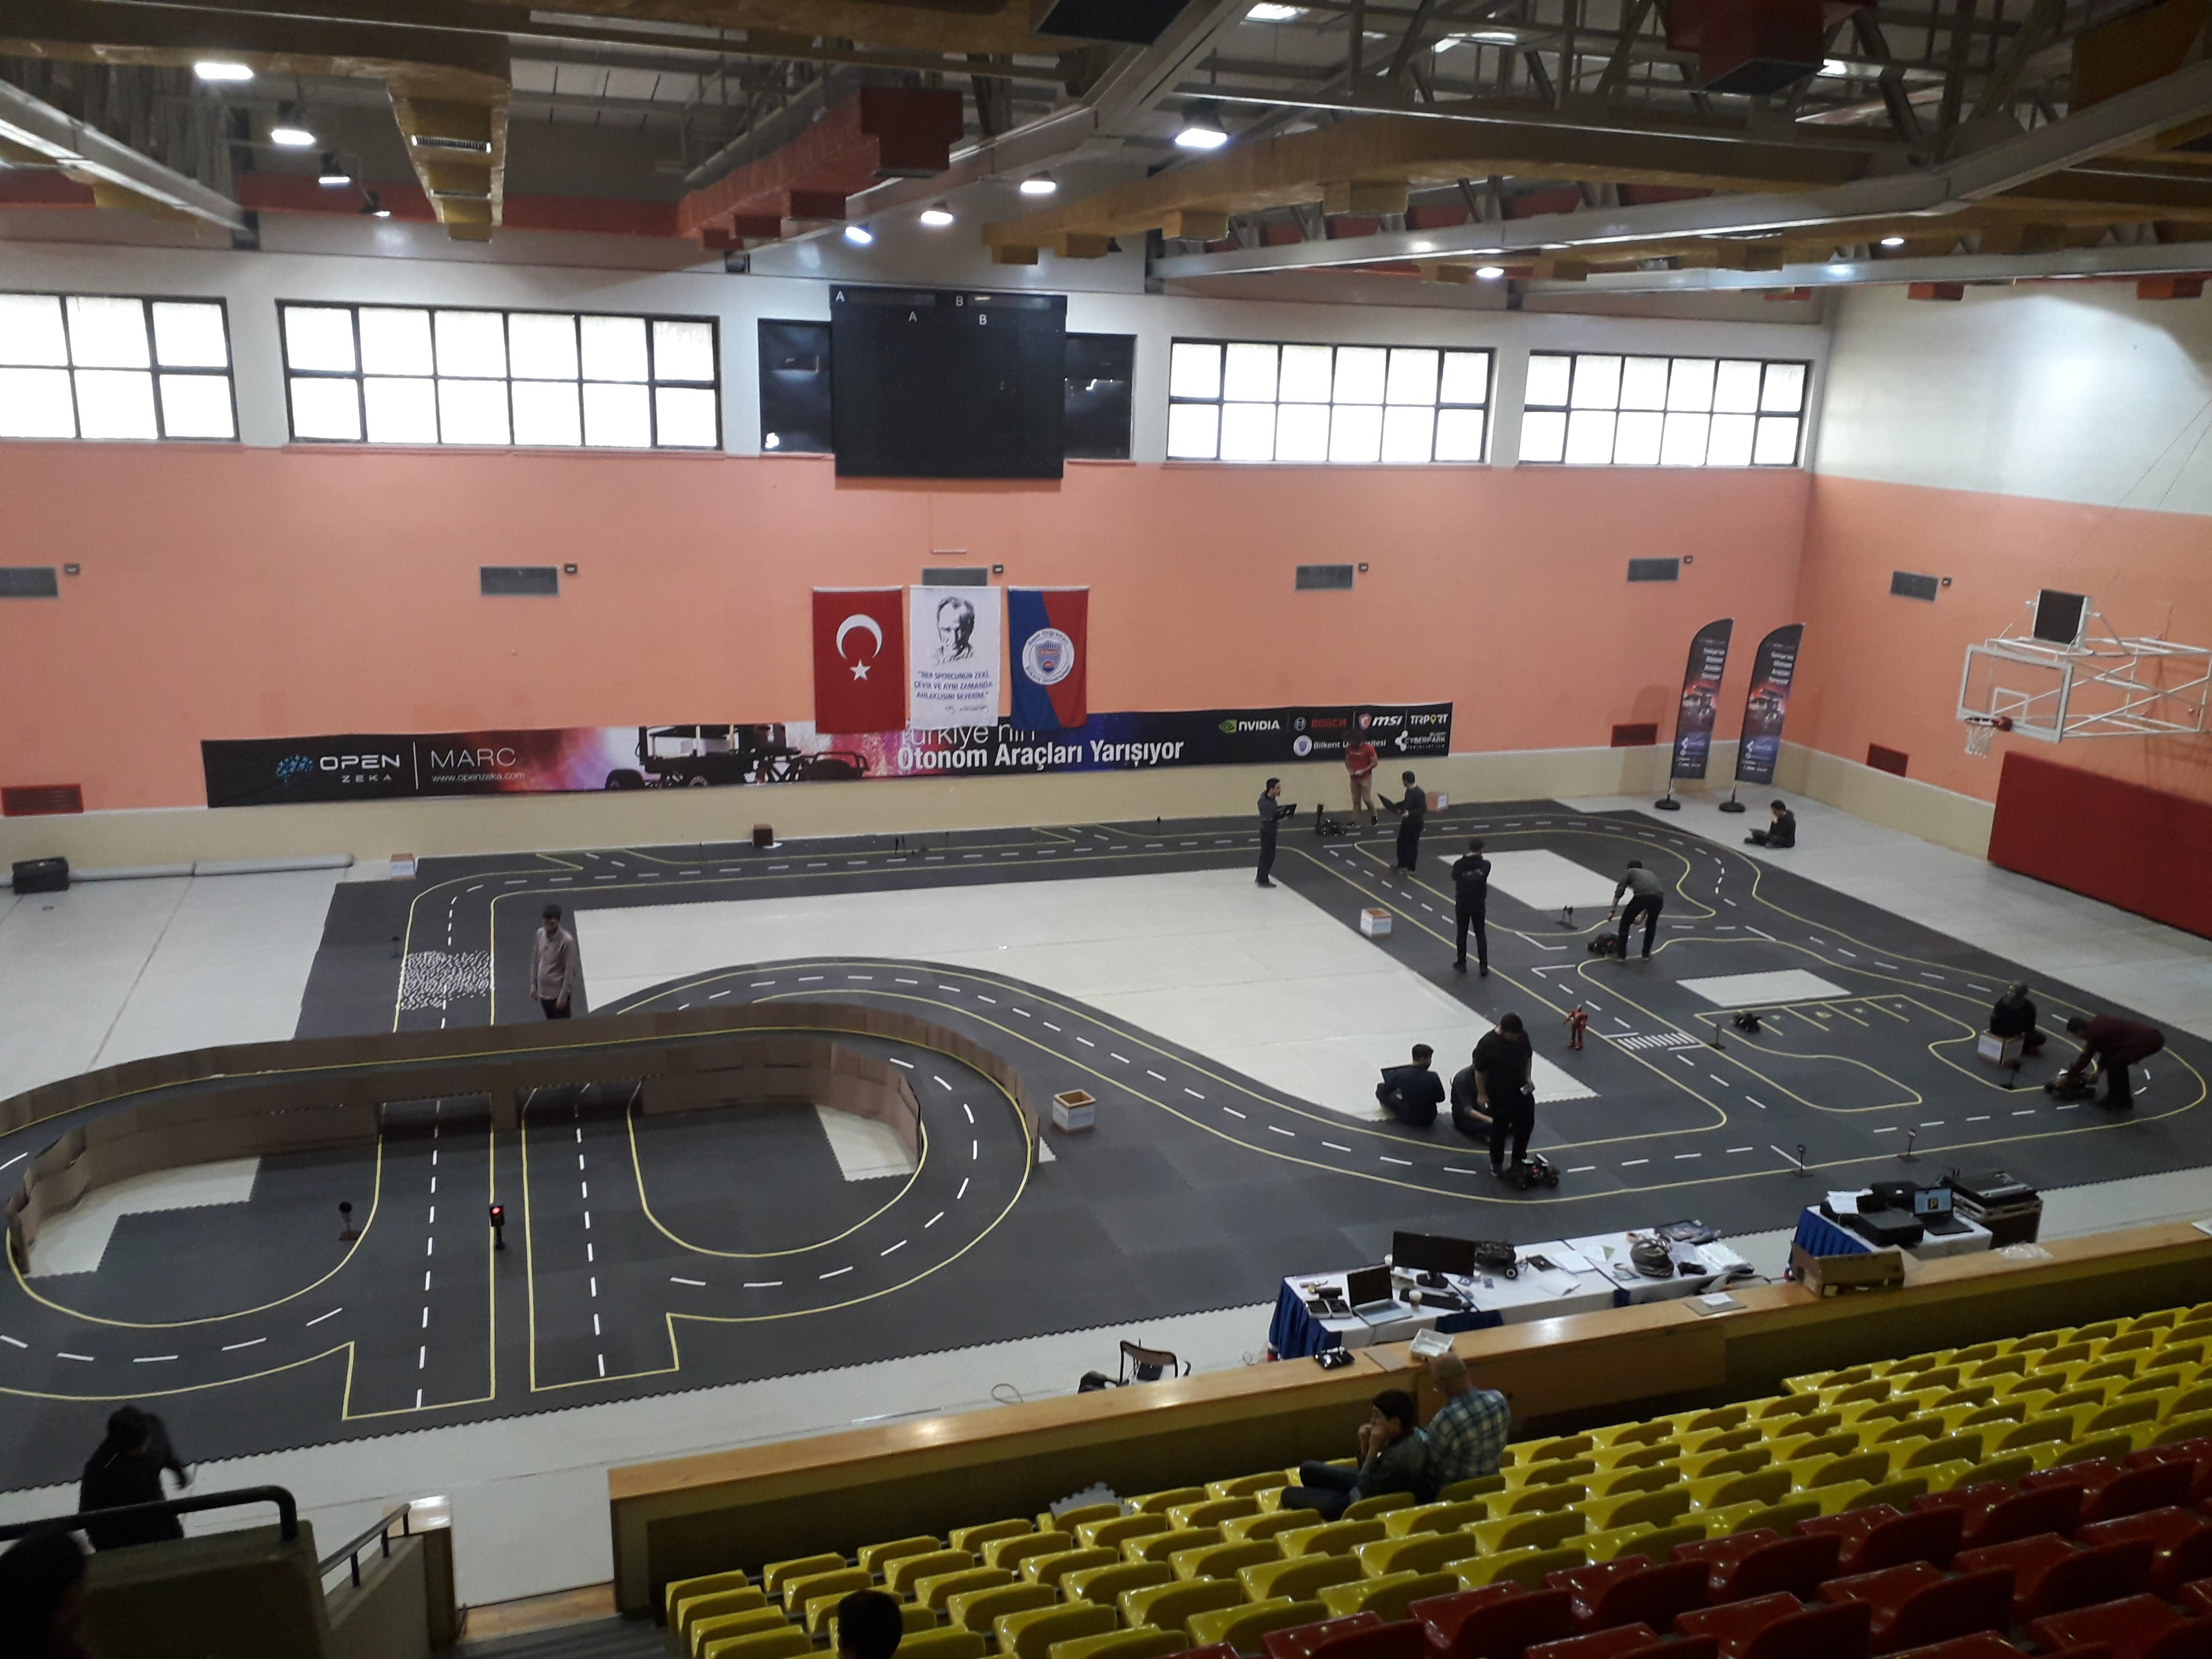
\includegraphics[width=.8\textwidth]{figures/openzeka-race-course.jpeg}
  \caption{OpenZeka 2019 MARC race course.}
  \label{figure:openzeka-race-course}
\end{figure}

\begin{figure}[h]
  \centering
  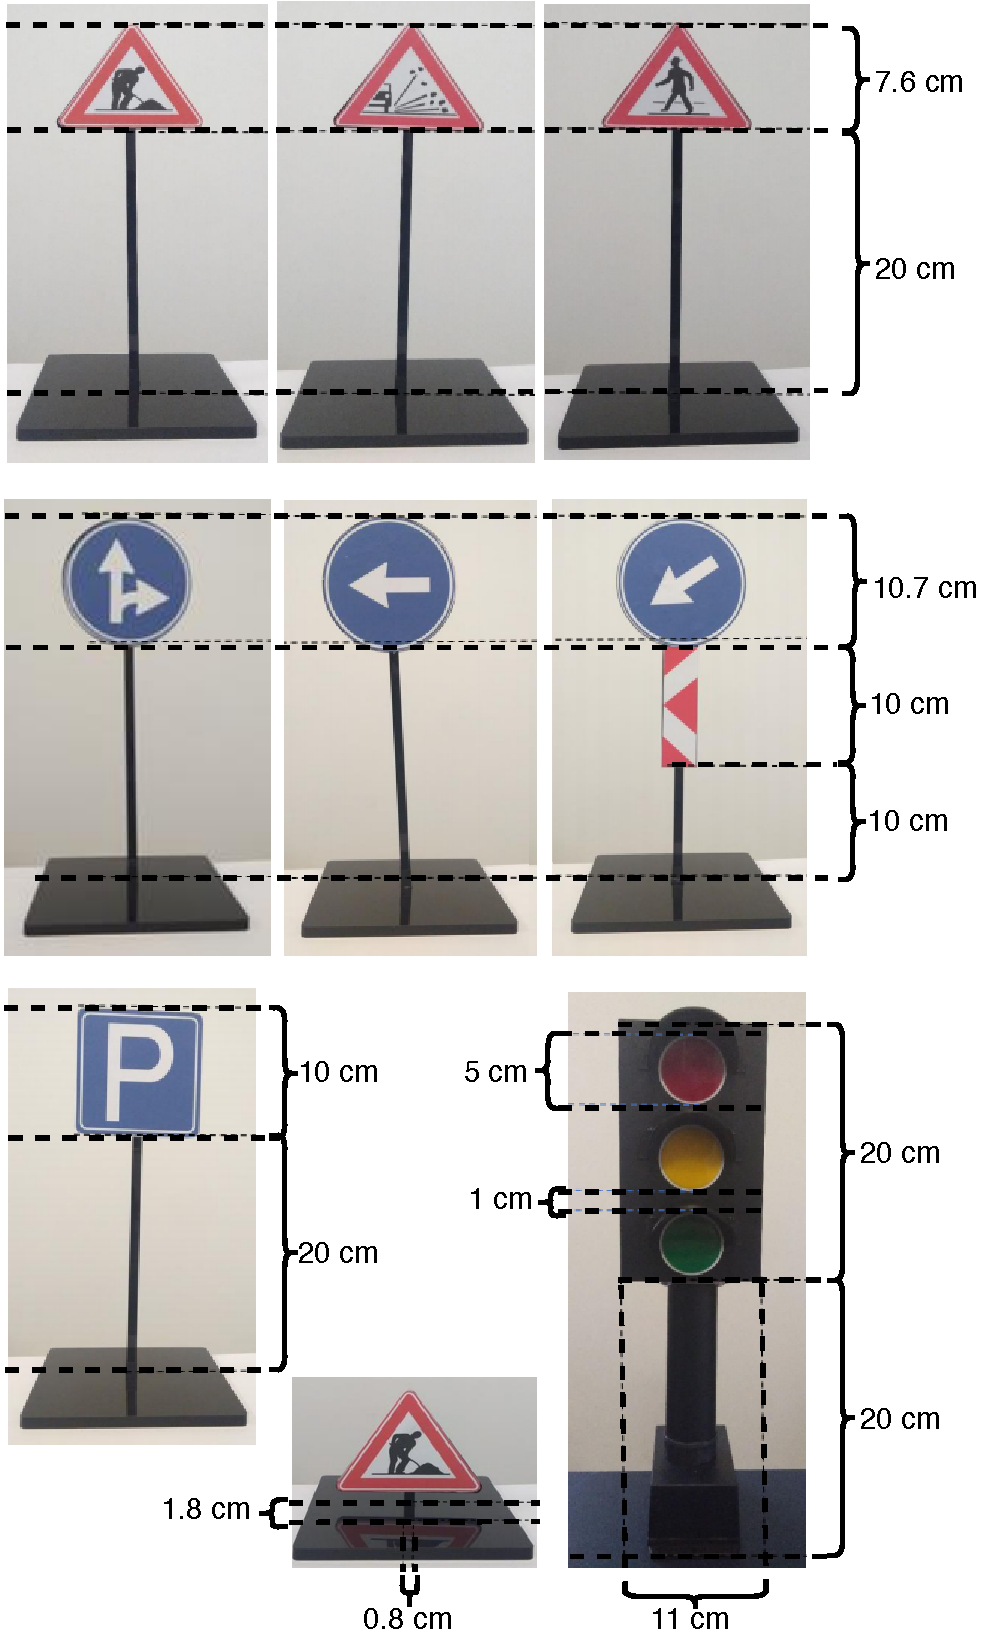
\includegraphics[width=.8\textwidth]{figures/openzeka-traffic-signs.pdf}
  \caption{Traffic signs and light specifically design for mini cars by
  OpenZeka.}
  \label{figure:openzeka-traffic-signs}
\end{figure}

\section{Contributions}

The main contribution of our study is as follows:

\begin{itemize}
  \item \textbf{Pixel classification dataset for mini cars:} Existing traffic
    scene datasets exclusively for real-scale cars \cite{Huang2018TheAD,
    Cordts2016TheCD, Geiger2012AreWR, Neuhold2017TheMV}. This poses a
    difficulty for on-road testing of the novel methods on mini-cars. We
    present a dataset with pixel-level annotations for mini cars.
  \item \textbf{Extended traffic sign and signal classification dataset:} We
    merge existing traffic sign classification datasets
    \cite{Timofte2009MultiviewTS, Stallkamp2012ManVC, Shakhuro2016RussianTS,
    Serna2018ClassificationOT, MaldonadoBascn2007RoadSignDA} for our scenarios
    and semi-automatically extend the dataset by cropping the segmented sign
    regions from our left camera images.
  \item \textbf{Development of a lane detector:} We build our lane detector on
    the approach proposed in \cite{Meyer2018DeepSL}. This approach essentially
    segments the road into ego lane, parallel lane, and opposite lane. It then
    extracts a center line for the ego lane. For our scenarios, we skip the
    opposite lane and further segment the parallel lane into right and left
    lanes.  Unlike \cite{Meyer2018DeepSL}, we are interested in finding center
    line curves for ego lane and also the neighboring parallel lanes. Our
    apprach saves us from analyzing the parallel lane pixels for right and left
    categorization for the curve estimation.
  \item \textbf{Local optimal trajectory planner for structured environments:}
    It is common that state-of-art autonomous vehicles relies on detailed maps
    to provide a reference line to the local planner for structural
    environments (i.e., environments with explicit drivable corridors), often
    by means of a global planner \cite{Thrun2006StanleyTR,
    Montemerlo2009JuniorTS, Kato2018AutowareOB}. We implemented a Frenet
    optimal trajectory planner \cite{Werling2010OptimalTG} without a map using
    exclusively the online computed lane centers as a source of the reference
    line.
  \item \textbf{Decomposed architecture for autonomous driving:} Autonomous
    vehicle architectures span wide range of computer science research areas
    including but not limited to computer vision, path planning, automata
    theory, control theory, and distributed systems.  Each of these areas comes
    with many problems and various alternative solutions to those problems. We
    put together a decomposed architecture with a selected set of solutions
    from different domains.
\end{itemize}

\section{Organization}

The organization of this thesis as follows. Chapter 2 discusses various
autonomous driving approaches and algorithms often used in search of autonomy
hightlighting their advantages and disadvantages.

Chapter 3 presents our hardware configuration and software architecture at a
high level. In Chapter 3, we also introduce our simulation environment that
accelerated the development and verification processes while implementing the
software components.

Chapter 4 provides a detailed description of our scene interpretation module in
which we implement perception and behavior planning capabilities of the car.
First, We present our segmentation model which is used to parse the current
scene into lanes and traffic signs. Second, we introduce our lane center line
extraction method based the parsed lane semantics. Third, we discuss our
traffic sign classification approach over the sign locations proposed by
segmentation model. Fourth, we review our obstacle detection method. Finally,
we explain our behavioral layer that implements a hierarchical finite state
machine that regulates the decisions made by the car based on the perception
capabilities.

Chapter 5 is dedicated to our trajectory planner and control algorithms. We
start with introducing Frenet frame on a lane segment and then we explain how
we plan an optimal trajectory based on the lane center lines provided by scene
interpretation module. In the second half of this chapter, we derive pure
pursuit algorithm that computes steering commands to execute our optimal
trajectories.

Chapter 6 presents our datasets, experiments, and results. In Chapter 6, we
evaluate our segmentation and classification models. Then, we demonstrate the
actions our car takes in response to various traffic scenarios.

Chapter 7 concludes our arguments by summarizing our approach to autonomous
driving with its limitations and suggesting directions for future work.

\chapter{Related Work and Background}
\label{chp:b2}

In this chapter, we review prominent autonomous driving architectures together
with the algorithms they are composed of. Along the way, we also briefly
discuss the historical development of self-driving cars, particularly two most
significant self-driving car competitions that paved the way for today's
driverless car technology, namely DARPA Grand Challenge and DARP Urban
Challenge.

In DARPA Grand Challenge 2004, no team saw the finishing line of of the race
course out of 15 teams. In DARPA Grand Challenge 2005, Stanley, a robot car
developed by Stanford Racing Team, was the first car to complete the race
course.  Thrun et al. \cite{Thrun2006StanleyTR} presents the details of the
competition rules and the software design of Stanley. According to Thrun et
al., a description of the race course was given to the participants in a
DARPA-defined format, RDDF two hours before the race. The RDDF contained a list
of longitudes, latitudes, road segment widths and a list of speed limits
associated with the road segments. In addition, the autonomous cars didn't need
to deal with dynamic obstacles.

Author states that Stanley's software is designed as a data processing pipeline
and processing nodes communicate through a publish/subscribe mechanism. Stanley
localizes itself on the RDDF by incorporating data from GPS, GPS compass, IMU,
and wheel encoders with UKF at 100 Hz. It performs terrain analysis based on
laser sensors and camera. For both data sources, the team automatically creates
datasets through human driving and apply machine learning algorithms to
classify the terrain into drivable and nondrivable regions. For the laser
readings, a set of parameters such as obstacle height threshold and acceptance
probability along with the Markov model parameters that capture the process and
measurement noise covariances are learned in a discriminative fashion by
coordinate ascent algorithm.

As opposed to laser terrain analysis, Stanley uses generative learning
algorithm for camera based terrain analysis. Drivable quadrilaterals ahead of
the vehicle extracted using the laser data is projected into the camera image.
The pixels inside the quadrilateral are then used as training samples. From
these samples, Stanley learns and maintains a database of Gaussians in RGB
space that corresponds to wide variety of drivable surfaces. The reach of a
laser range is smaller than that of the camera. On the other hand, vision based
terrain analysis is susceptiple to olcor and lighting changes in the
environment.  Therefore, Stanley uses the laser based terrain analysis for
steering control and vision based analysis for speed control so that the vision
module acts as an early warning system when an obstacle is ahead but not within
the range of the lasers.

Because the detailed race track is provided in RDDF, Stanley's main focus is
local obstacle avoidance rather than global planning. Though there are no lanes
in the course, Stanley introduces lateral offsets over the base trajectory
which is a smoothed path extracted from RDDF. Stanley basically plans a
trajectory to smoothly change into a lateral offset within the drivable path
for obstacle avoidance similar to the lane change in highway driving. The
planner finds a minimum cost trajectory by evaluating a cost function which is
subject to kinematic and dynamic constraints of the vehicle, distance to
obstacles, distance from the center of the road, and being on the course
corridor.

Stanley uses its own steering control algorithm to track the optimal trajectory
proposed by the path planner. Relying on the geometrical relation between the
car pose and the trajectory, Stanley minimizes the cross-track error, which
measures the lateral distance between the center of front axle and the nearest
point on the target trajectory. The geometrical relation is illustrated in
Figure \ref{figure:stanley-control}.

\begin{figure}[h]
\centering
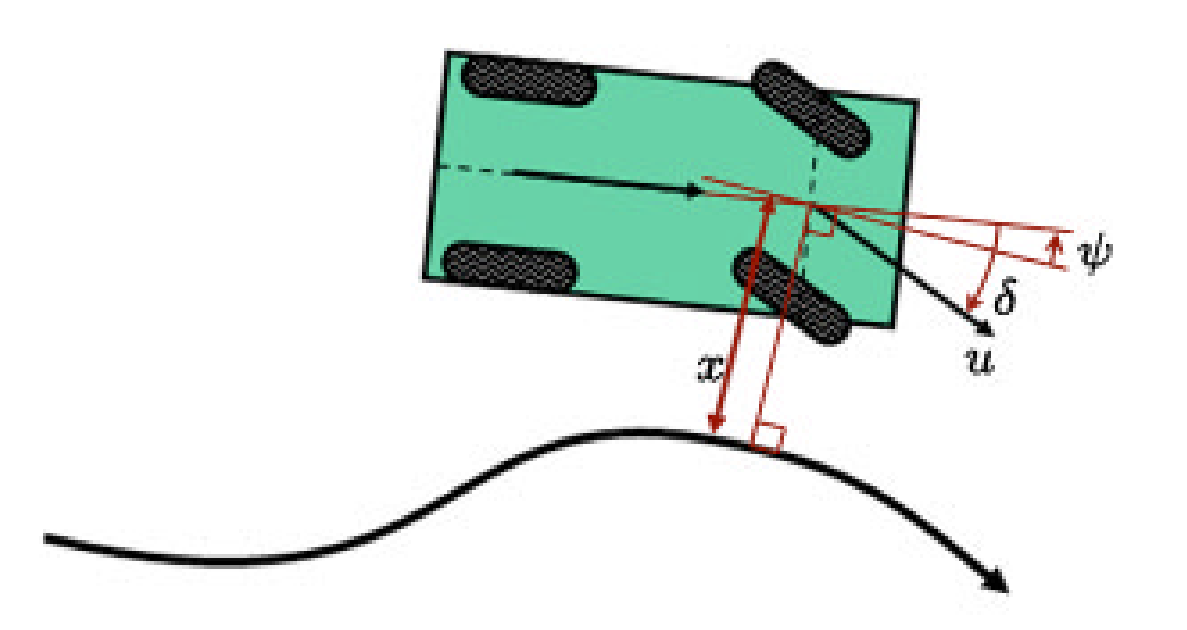
\includegraphics[width=.8\textwidth]{figures/stanley-control.png}
\caption{The geometrical relation between the trajectory and the car used by
Stanley controller algorithm. Taken from \cite{Thrun2006StanleyTR}.}
\label{figure:stanley-control}
\end{figure}

Nonlinear feedback function of cross-track error is given by Equation
\eqref{eq:stanley-control}.

\begin{equation}
    \delta(t) = \psi(t) + \arctan\frac{kx(t)}{u(t)}\ \textbf{,}
\label{eq:stanley-control}
\end{equation}

where $k$ is a gain parameter, $u(t)$ is the car speed, and $\psi(t)$ denotes
the orientation of the nearest trajectory segment relative to the car's
orientation. The intuition behind the controller is that as the cross-track
error $x(t)$ increases, the controller produces stronger steering angle
$\delta(t)$ towards the trajectory.  Likewise, as the speed $u(t)$ increases,
the controller avoids sudden strong maneuvers. Hoffmann et al. studies the
Stanley controller algorithm in greater detail in
\cite{Hoffmann2007AutonomousAT}.

In 2007, DARPA Urban Challenge took place. Montemerlo et al. \cite{cite1}
presents the competition details and the software architecture of Junior,
Stanford's another robot car and the second best car in the challenge. This
time rules were more complex including overtaking parking or moving vehicles,
precedence handling at intersections possibly with stop signs, merging into
fast moving traffic, left turns, parking and U-turns when the road is
completely blocked. Participants were provided with a road network description
file or RNDF which contained lane information, stop signs, parking lots, and
special checkpoints. In addition, the teams were also provided with a high
resolution aerial image of the race course so that they can further improve the
RNDF. In the competition, the vehicles were given multiple missions as a
sequence of checkpoints in the RNDF.

Like Stanley, Junior's software software architecture is made of sensor
interfaces, perception, navigation, and drive-by-wire interfaces at the core.
The design is again based on data processing endpoints communicating with
publish/subscribe pattern. Unlike Stanley, Junior's modules are far more
advanced.  Junior's perception module segments the environment data into moving
vehicles and static obstacles. Its navigation features a global path planner
based on dynamic programming to find an optimum path to the mission checkpoints
from the current location of the car. Moreover, the navigation module handles
different driving scenarios with different planning algorithms.

It performs free-form navigation in parking lots, at U-turns or whenever the
car gets stuck for extended period of time. The free-form planner is
specifically developed for Junior and named hybrid A* by the Stanford Racing
Team. Hybrid A* associates discrete search space of regular A* with a
continuous state by performing forward simulations with different steering
angles and computes a score based on the continuous state. The continuous state
is represented by x-y position of the car, heading direction, and the
direction, either forward or reverse. Whereas the path found by the regular A*
and Field D* algorithms cannot be executed due to their discrete nature, hybrid
A* can find executable paths that the nonholonomic constaints of the vehicle.
Hybrid A* uses dual admissible heuristics. One heuristic is nonholonomic
without obstacles, and the other is holonomic with obstacles. Once a solution
is found, it is smoothed for a better driving experience. Extensive study and
experiments show that hybrid A* produces near-optimal solutions
\cite{Dolgov2010PathPF, Petereit2012Application}. Figure
\ref{figure:hybridastar-comparison} demonstrates the difference between regular
A*, Field D*, and hybrid A* algorithms.

\begin{figure}[h]
\centering
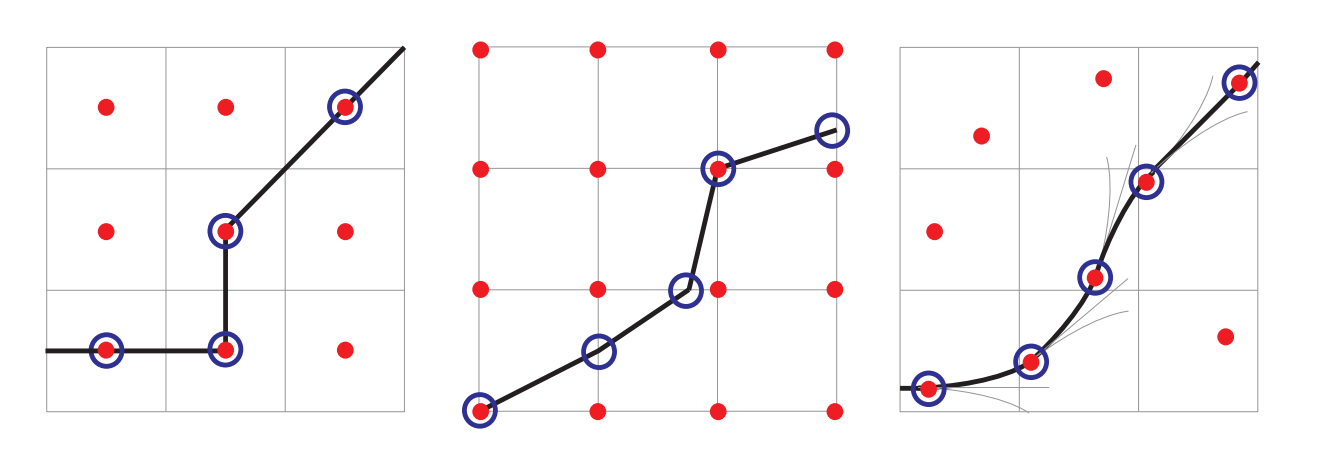
\includegraphics[width=.8\textwidth]{figures/hybridastar-comparison.png}
\caption{Left: Regular A* solutions passes through only the center of grids.
    Center: Field D* solutions can have arbitrary linear paths from cell to cell.
    Right: Hybrid A* associates a continuous state with each cell and compute a
score for the continuous state. Taken from \cite{Dolgov2010PathPF}.}
\label{figure:hybridastar-comparison}
\end{figure}

Junior uses a different planner for normal on-road navigation. It performs
internal simulations with different steering parameters. The internal
simulations generate candidate trajectories according a reference path. This
reference path is essentially the smoothed center of the lane obtained from
RNDF. The planner evaluates the candidate trajectories by a cost function and
finally selects the best trajectory. The cost function also regulates the lane
change or overtaking behavior of Junior. When the right lane is blocked, the
car chooses to shift left. When the overtaking is complete, it steers back to
the right lane as it would be more costly to occupy the left lane.

Driving behavior of Junior is governed by a hierarchical finite state machine.
The state machine decides on the U-turns, handles intersection precedence and
stop signs, prevents the car from getting stuck, switches to parking navigation
in a parking lot or chooses the true planner for the current scenario in
general.

Werling et al. \cite{cite14} reports that they generated optimal trajectories
in Frenet frame and tested it on Junior without obstacles. They also present
their obstacle avoidance experiments in simulation. In their method, they
suggest integrating trajectory generation with a behavioral layer that decides
on the high level as to whether the car should keep a constant velocity, follow
the car in front with a constant distance, merging into traffic or stoping at a
point. Figure \ref demonstrates a velocity keeping instance in this approach.

\begin{figure}[h]
\centering
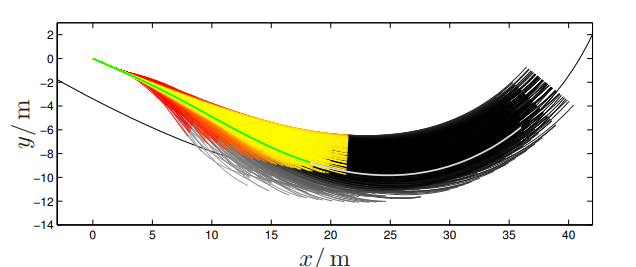
\includegraphics[width=.8\textwidth]{figures/frenet-velocity-keeping.png}
\caption{An exmaple optimal trajectory generated in Frenet frame in velocity
    keeping mode. Colors from red to yellow represent increasing lateral cost.
    Colors from grey to black represent increasing longitudinal cost. Green and
    light grey colors represent the optimal trajectory, which leads the car to
    the reference line and desired speed. Taken from \cite{cite14}.}
\label{figure:autoware}
\end{figure}

Yoneda et al. \cite{cite15} further extends the method in \cite{cite14}
introducing an additional adjust mode while switching from velocity keeping
mode or cruise mode to distance keeping in an affort to eliminate strong
acceleration and deceleration during the mode switching in the quest of a more
natural driving experience.

Fast forward to the present day, Autoware \cite{Kato2018Autoware0B}, being one
of the modern open source self-driving car platform is based on ROS
\cite{cite3}. ROS is a commonly used, extendible, component based, higly
modular middleware framework with many reusable packages and visualization
tools that dramatically accelerated today's robot development and prototyping
processes.  Unsurprisingly, publish/subscribe mechanism is at the core of ROS
communication patterns. Autoware implements perception, decision-making,
planning and path tracking capabilities. Figure \ref{figure:autoware}
illustrates the the Autoware architecture at a high level.

\begin{figure}[h]
\centering
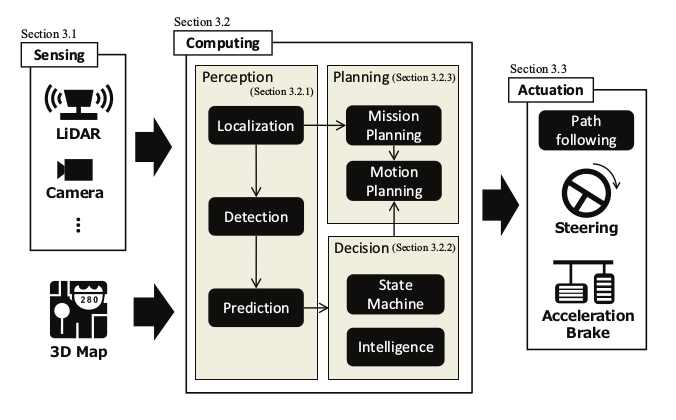
\includegraphics[width=.8\textwidth]{figures/autoware.png}
\caption{Autoware high level architecture and data flow. Taken from
    \cite{Kato2018Autoware0B}.}
\label{figure:autoware}
\end{figure}

Perception capabilities are made of localization, detection, and prediction
modules. For the localization, Autoware relies on high definition 3D maps. It
localizes itself appling scan matching between the 3D map and LiDAR scans.
Therefore, a 3D map of the environment should be created beforehand using SLAM
technologies, in which scan matching is applied against previous LiDAR scans
instead of a 3D map such that a transformation between the LiDAR scans are
obtained and a cumulative point cloud is continually updated. Other perception
modules are also rely on the localization. For example, the car is localized in
the 3D map, it projects 3D map fatures into the front view camera images to
define a ROI for traffic light detection and classification in order to
eliminate full image search on every image frame. The detection module supports
both deep learning and traditional image processing and machine learning
techniques. It features YOLO2 \cite{Redmon2016YOLO9000BF} and SSD
\cite{Liu2016SSDSS} models for detecting objects in the traffic such as traffic
signals, pedestrians, and other vehicles. In the prediction module, Autoware
associates detected objects with time, so that it estimates trajectories for
the moving objects which are then used in the planning modules. Based on the
perception modules, Autoware makes decisions in response to the environmental
changes. The decision-making scheme is captured in a finite state machine
similar to Junior.

Autoware features two set of planners, a mission planner and motion planners.
The mission planner is responsible for a rough global path from the current
location to the destination in the map. Motion planners, on the other hand,
generates local trajectories taking the global plan as a reference. In
unstructured environments such as parking lots, hybrid A* is used similar to
Junior. For well-structured environment scenarios such as navigating on the
lanes, state lattice based algorithms are preferred. Pivtoraiko et al.
\cite{Pivtoraiko2009DifferentiallyCM} introduces space lattice based planning.
The state lattice is made of motion primitives of a specific car. The motion
primitives are generated offline by a precise trajectory generator respecting
the mobility model of the vehicle such as steering limits and wheelbase. Then,
the lattice search space could be search by D* algorithms for optimal
trajectories. This method also successfully used in DARPA Urban Challenge by
the winner vehicle, Carnegie Mellon University's Tartan Racing for navigating
in unstructural environments \cite{Urmson2007TartanRA}. Figure
\ref{figure:state-lattice} illustrates a state lattice. McNaughton et al.
\cite{McNaughton2011MotionPF} later extended this approach and applied it to
structural environments.

\begin{figure}[h]
\centering
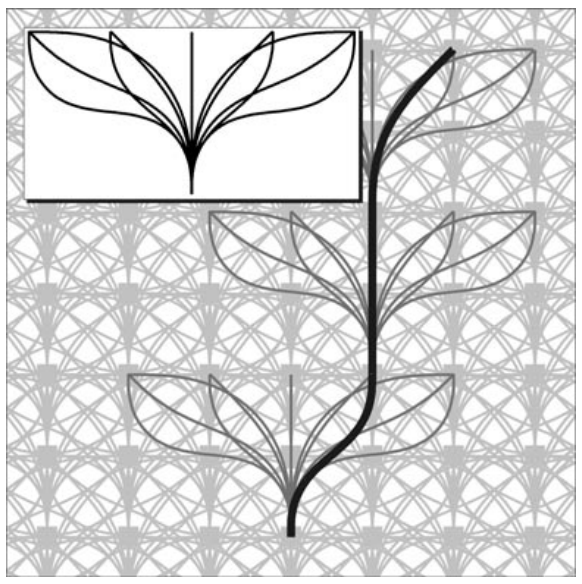
\includegraphics[width=.8\textwidth]{figures/state-lattice.png}
\caption{An example state lattice without reverse motions. Taken from
\cite{Pivtoraiko2009DifferentiallyCM}.}
\label{figure:state-lattice}
\end{figure}

Autoware uses pure pursuit controller to generate low level steering commands
to execute the given trajectory from the motion planners. Kim et al.
\cite{cite18} studies the controller with its geometrical derivation and also
gives some useful pointers on tuning.

Backed by Baidu, Apollo is another open source autonomous driving platform with
its giant dataset \cite{Huang2018TheAD}. Similar to other other decompositioned
architectures, Apollo is also made of localization, perception, prediction,
routing, motion planner, and vehicle control components as shown in Figure
\ref{figure:apollo}. Like Autoware, Apollo also relies on high definition 3D
maps for location and perception \cite{Fan2018BaiduAE}.

\begin{figure}[h]
\centering
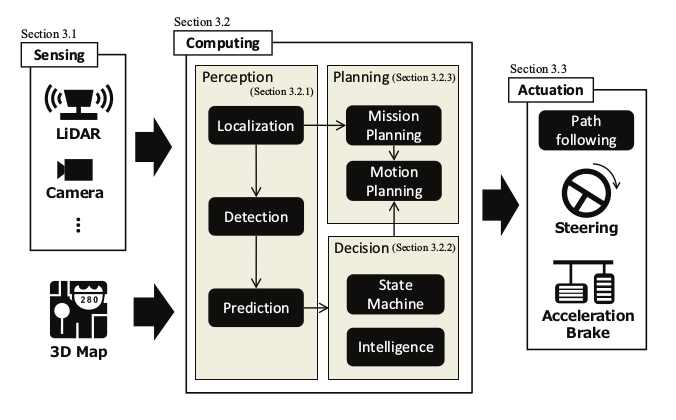
\includegraphics[width=.8\textwidth]{figures/autoware.png}
\caption{Apollo high level architecture and data flow. Taken from
    \cite{Fan2018BaiduAE}.}
\label{figure:autoware}
\end{figure}

The routing component finds a global plan from the current location
to a destination in the map like previous architectures; however, Apollo's
lane-based motion planner is quite different. Apollo does not directly use
this global plan as a reference path for trajectory generation, but rather it
generates multiple lane level reference lines from it taking traffic
regulations (e.g., traffic signs, signals and lane markings) and safety
measures into account.  During lane level motion planning, Frenet frames are
constructed based on the given reference lines.  Lane level path and speed
optimizers generate the optimal trajectories in Frenet frame for each lane.
Finally, a trajectory decider chooses the best trajectory for the maneuver
given the cost of each trajectory, car status, traffic regulations.  This
approach allows for dealing with different traffic regulations that apply for
different lanes of the same road \cite{Fan2018BaiduAE}.

A different approach to autonomous cars is to learn a mapping from input images
to steering angle and speed commands in an end-to-end manner. Bojarski et al.
\cite{Bojarski2016EndTE} were the first to apply this method to a real-sized
car with the modern deep learning advancement. They collected 72 hours data
with different cars in different weather and lighting conditions from various
places. For the data acqusition, they installed three cameras on the car behind
the windshild and recorded timestamped videos from the left, right and center
cameras along with the steering commands controlled by a human driver. During
training, they agumented the dataset by random shifting and rotating the images
and adjusting the recorded commands accordingly. The trained model then
successfully steered the car by using the images only from the central camera.
Figure \ref{figure:end-to-end-network} demonstrates the training and testing
steps of this approach.

\begin{figure}[h]
  \centering
  \begin{subfigure}[b]{0.4\linewidth}
      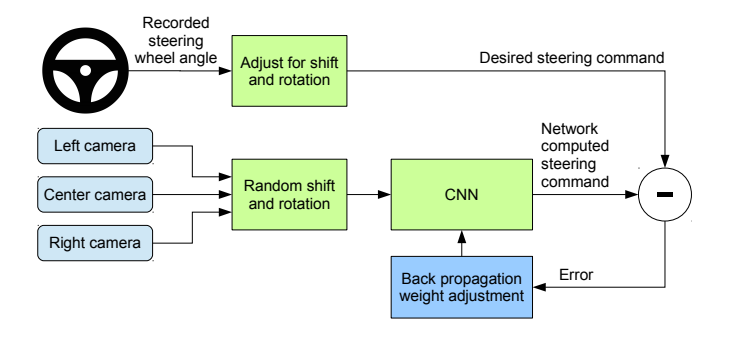
\includegraphics[width=\linewidth]{figures/end-to-end-training.png}
    \caption{}
  \end{subfigure}
  \begin{subfigure}[b]{0.4\linewidth}
      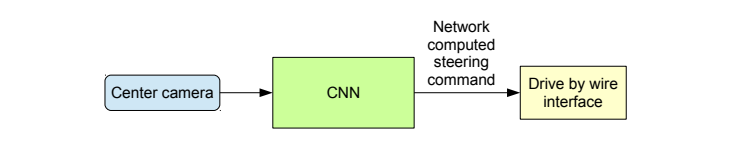
\includegraphics[width=\linewidth]{figures/end-to-end-inference.png}
    \caption{}
  \end{subfigure}
  \caption{(a) End-to-end training scheme. (b) Steering command inference from
  raw camera images. Taken from \cite{Bojarski2016EndTE}.}
  \label{figure:end-to-end-network}
\end{figure}

Bechtel et al. \cite{Bechtel2017DeepPicarAL} relicated the work
\cite{Bojarski2016EndTE} with a small-scale, low-cost platform using a web
camera and Raspberry Pi 3 for inference. They conducted successful experiments
in a specially built test course for the RC car.

Do et al. \cite{Do2018RealTimeSC} also implemented a similar approach in
another RC car platform using Pi camera and Raspberry Pi 3 for inference.
Instead of learning steering angles in a regression model, they learned a
steering angle probability for discretized steering angle space. In addition to
basic lane following, they also learned to turn left or right when the
corresponding traffic sign is encountered. The traffic sign diameter was 15 cm
in their experiments.

There are several traffic scene segmentation segmentation datasets available.
Currently, the largest and the most comprehensive is ApolloSpace
\cite{Huang2018TheAD}. It is followed by Cityscapes \cite{Cordts2016TheCD},
KITTI \cite{Geiger2012AreWR}, and Mapillary Vistas \cite{Neuhold2017TheMV}
datasets. Because these datasets are created for real-sized cars on the real
roads, they were not much useful for us, so we had to create our own
segmentation dataset. The existing traffic sign and signal classification
datasets \cite{cite11, cite12, Shakhuro2016RussianTS,
Serna2018ClassificationOT, MaldonadoBascn2007RoadSignDA}, on the other hand,
was useful to train an initial classifier as they are mostly independent of the
scene and car size.

Sakai et al. \cite{cite18} presents a collection of various autonomous
navigation algorithms implemented in Python Programming Language in their basic
forms. The collection includes aforementioned hybrid A*, frenet optimal
trajectory planner, state lattice planner, stanley controller, and pure pursuit
controller algorithms.

Unlike Stanley, Junior, Autoware and Apollo, we don't have a detailed map of
the driving course. As a result, our best option is to follow the lanes unless
a traffic sign or another conditions mandate otherwise. For the same reason, we
have to create our reference paths for our local trajectory generation either
from the online detected lane centers or according to the traffic regulations.
Meyer et al. \cite{cite9} studies semantic lane segmentation for mapless
driving, which bears similaries to our lane detection approach.  Autohors
motivation is the fact that as the high definition maps quickly gets out of
date due to constructions an autonomous car should also be able to perform
basic navigation tasks without a precise map, but possibly with a course map,
specifically for intersections. They start with creating their own dataset by
extending Cityscape \cite{Cordts2016TheCD}. Their approach is to annotate the
road surface as ego lane, parallel lane, and opposite lane and learn these
regions with a semantic segmentation model.

Stanley controller algorithm is weak to discontinuities along the trajectory as
it directly drives towards the closest point on the trajectory. Stanley and
Junior guarantees a smooth trajectory by smoothing already known center
reference lines or post processing the output of hybrid A*. We cannot guarantee
a smooth path as we use discontinuous predefined path in response to traffic
signs and signals or due to instantaneous segmentation errors in the lane
detection.  Conversely, as pure pursuit controller drives along an arc it is
less likely to be affected by discontinueties.

\chapter{Architectural Overview}
\label{chp:b3}

In this chapter, we introduce our proposed architecture of the mini driverless
car with its hardware and software components. We also present our simulation
environment, which was implemented to speed up the development and
verification processes.

\section{Hardware Configuration}

Autonomous cars are equipped with a powerful central computer, actuators and
many sensors such as IMU, Camera, and LIDAR. Our mini driverless car also has
the equivalent hardware components as shown in Figure
\ref{figure:hardware-configuration}. Details of these components are given in
Table \ref{table:hardware-configuration}.

\begin{figure}[h]
\centering
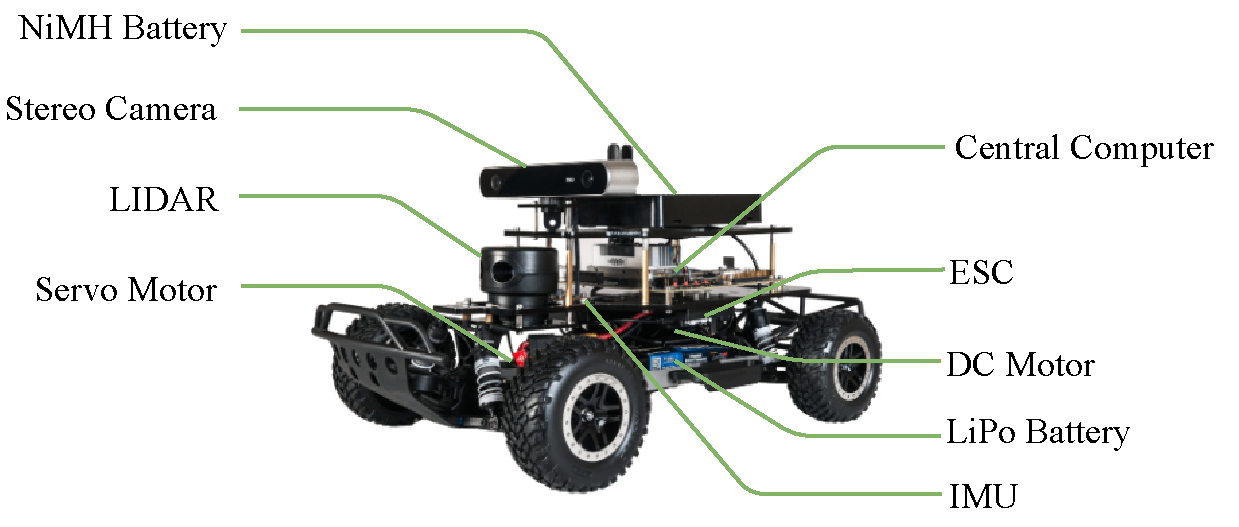
\includegraphics[width=.8\textwidth]{figures/hardware-configuration.pdf}
\caption{Hardware components on the mini driverless car.}
\label{figure:hardware-configuration}
\end{figure}

\begin{table}[h]
\caption{Mini driverless car hardware configuration details.}
\label{table:hardware-configuration}
\resizebox{\textwidth}{!}{\begin{tabular}{||c c||}
 \hline
 Component & Description \\ [0.5ex]
 \hline\hline
 Vehicle & TRAXXAS SLASH 4X4 PLATINUM EDITION \\ 
 \hline
 Central Computer & NVIDIA Jetson TX2 Developer Kit \\
 \hline
 Stereo Camera & Stereolabs ZED Camera \\
 \hline
 2D LIDAR & Scanse Sweep LIDAR \\
 \hline
 ESC & Vedder Electronic Speed Controller \\
 \hline
 IMU & SparkFun 9 DoF Razor IMU M0 \\
 \hline
 USB3.0 Hub & USB 3.0 7-Port Hub with 2 Charging Ports UH720 \\
 \hline
 Joystick & Logitech F710 Wireless Gamepad (940-000142) \\
 \hline
 LiPo Battery & 4200 mAh 7,4V 25C \\
 \hline
 NiMH Battery & MARC Power Lite 3400mAh 16V and 12V outputs \\ [1ex]
 \hline
\end{tabular}}
\end{table}

The central computer runs various sophisticated algorithms to fuse raw data
from sensors to achieve situational awareness, select the best possible action
accordingly, and finally send speed and steering angle commands to the ESC.  in
order to execute the action. The ESC generates necessary electronic signals
from the commands and feeds them to servo and DC motors to control steering
angle and speed, respectively. We replace the stock ESC that ships with the
vehicle with a different speed controller known as VESC, an open source ESC,
since it is highly configurable and thus supports full control at lower speeds
\cite{cite2}. The hardware setup also provides a joystick control in order to
acquire dataset from a human driver and take over the control during the
autonomous drive in case of an emergency. We use two different batteries to
power the vehicle.  While NiMH battery powers the central computer and sensors
through the USB 3.0 Hub, LiPo battery supplies current to the actuators as they
need a more consistent power source in both quality and quantity.

\section{Software Architecture}

We use Robot Operating System (ROS) \cite{cite3} to implement our architecture.
ROS defines notion of nodes and allows nodes to communicate through
publish/subscribe and reply/request mechanisms. Similar to \cite{cite1}, we
also rely on publish/subscribe mechanism for the data flow between our nodes.
Nodes subscribe to the message streams from other nodes. The result of the
computation of a node is then published to the other nodes. This asyncrononous
messaging alows the software to act as a data processing pipeline. The
architecture is roughly grouped into four modules.

\begin{itemize}
    \item \textbf{sensor interface --} The sensor interface reads raw data from
        individual sensors, converts them to meaningful engineering data, then
        feeds them to the other modules.
    \item \textbf{scene interpretation --} The scene interpretation module
        makes sense of the the the environment by finding traffic lanes,
        detecting obstacles, and classifying the traffic signs. Once the
        objects of interests are detected and classified, the module also
        locates the these objects in the real world coordinates with respect to
        car's body frame. Then it decides on a high-level behavior that best
        fits to its current perception of the environment such as keeping a
        lane or stopping on a red light.
    \item \textbf{navigation --} The navigation module first takes the
        kinematic constraints, traffic rules, and nearby obstacles into account
        and generates an optimal trajectory to realize the high-level behavior.
        Then it computes steering angle and speed values in order to follow the
        optimal trajectory as close as possible.
    \item \textbf{actuator --} A pre-configured firmware in the VESC converts
        steering and speed commands into electronic signals to drive the
        motors.
\end{itemize}

Figure \ref{figure:software-architecture} illustrates the overall data flow in
the software modules. Out of these modules, nodes in sensor interface and
actuator modules are already provided as ROS packages. They are not implemented
but configured within the scope of this thesis.

\begin{figure}[h]
\centering
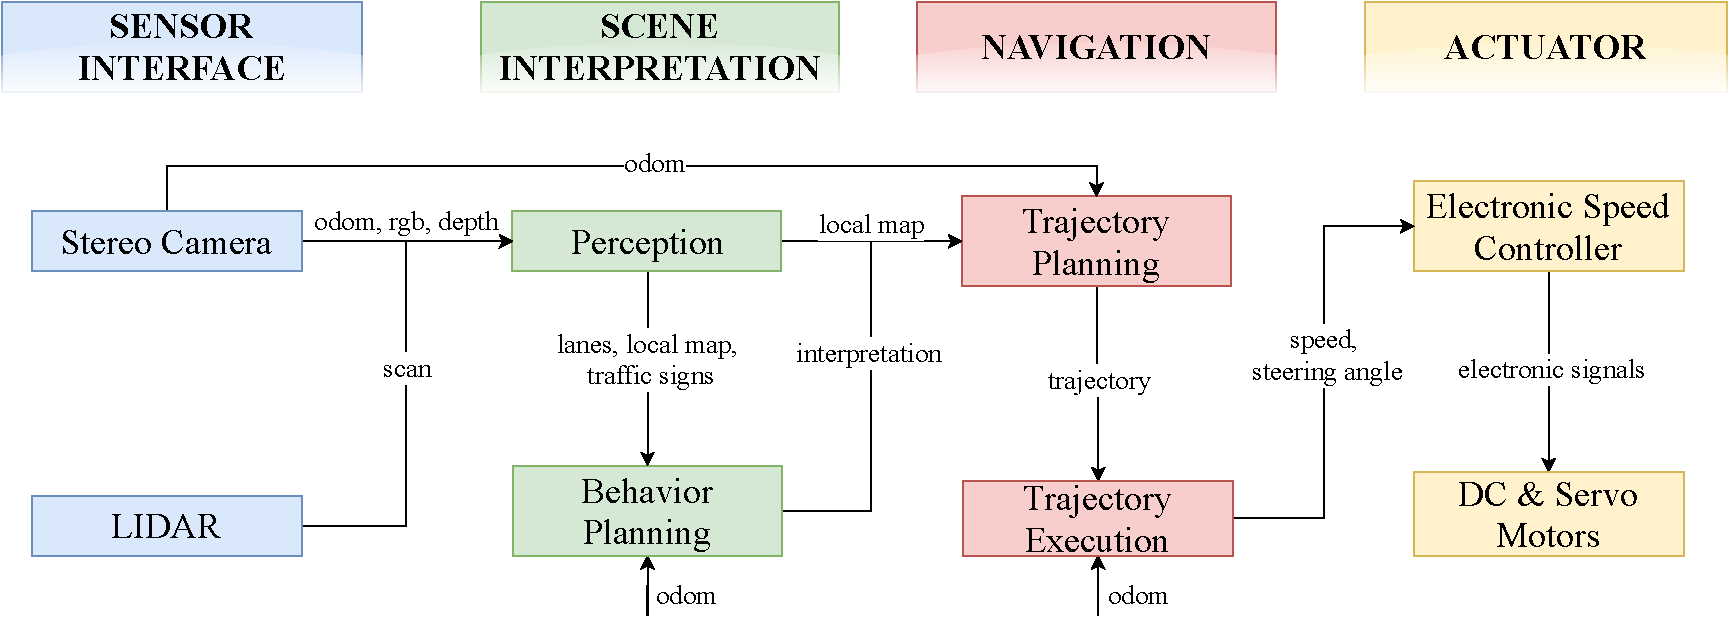
\includegraphics[width=.9\textwidth]{figures/software-architecture.pdf}
\caption{Software architecture overview.}
\label{figure:software-architecture}
\end{figure}

Zed camera node is configured to publish visual odometry, RGB, and depth topics
at the rate of 15 Hz. Message types flow through this topics are well-defined
in ROS. An odometry message contains position, orientation, linear and angular
velocities with respect to the starting point, i.e. with respect to the
odometry frame. RGB image message is a rectified color image from the left zed
camera, which is used for image segmentation and classification. Because zed
camera features stereo images, it can also publish a depth image, which is used
to locate the traffic signs with respect to the body frame.

LIDAR node is configured to provide scan data to the costmap nodes in the scene
interpretation module at 5 Hz rotational speed. The costmap nodes then
publishes local occupancy grid maps that indicate nearby objects. Scene
interpretation maintains two local maps in different sizes. The small map is
used in navigation module for collision avoidance.  The larger map is
internally used by the scene interpretation module for behavior planning to
guide the trajectory planner before the navigation module observe the
obstacles.

Behavior planner component decides if the car should stop or in which speed
range it should move, whether it should track the lanes or follow a predefined
path. At the end, the behavior planner captures the current desired
behavior in an interpretation message and publishes to the trajectory planner.

Trajectory planner subscribes to the odometry, 3x3 local map, and
interpretation topics so as to find a collision-free, kinematically feasible,
smooth, and optimal trajectory. The trajectory message contains waypoint
locations in the odometry frame and a recommended speed for each waypoint.

Finally, given the odometry and optimal trajectory, the trajectory execution
node computes steering angles to closely follow the optimal trajectory and
publishes the recommended speed and steering commands to the actuator module.

\section{Simulation Environment}

It is not always practical to try new ideas on the target platform for several
reasons. First, it is too risky to run an updated version of software in the
target platform as it would crash into an obstacle. Second, the batteries have
certain life time and we do not want to drain them for each immature update to
the code base. Third, deploying ad testing the software on the target is time
consuming. The last but not least, because running the software on the target
requires a large enough spacial area with various traffic signs, lanes, a
bridge and many other urban conditions, which we could barely afford a few, we
had no better option than creating a simulated environment.

We used Gazebo to model our simulation world and robot car. Figure
\ref{figure:simulation-environment} shows the simulated urban area. It
simulates every case in OpenZeka MARC 2019 except that we have to manually
replace red and green lights, and manually remove the pedestrian from the
scene.

\begin{figure}[h]
  \centering
  \begin{subfigure}[b]{0.4\linewidth}
      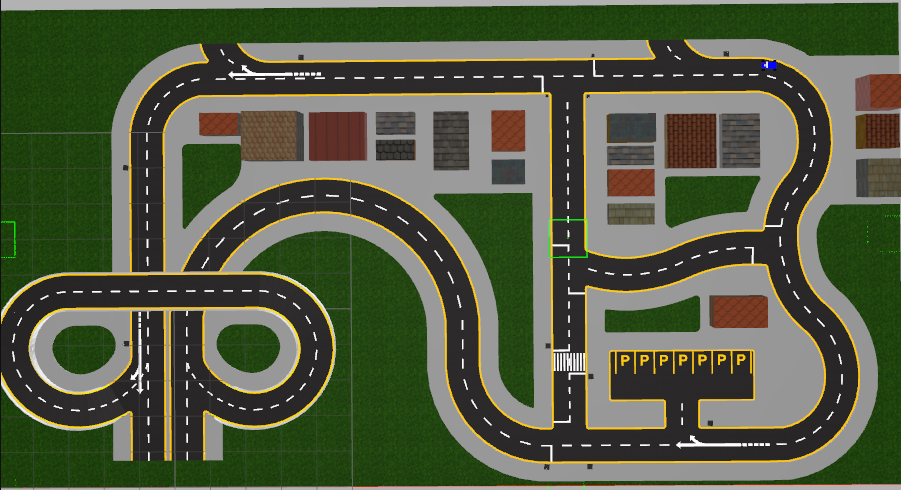
\includegraphics[width=\linewidth]{figures/simulation-environment1.png}
    \caption{}
  \end{subfigure}
  \begin{subfigure}[b]{0.4\linewidth}
      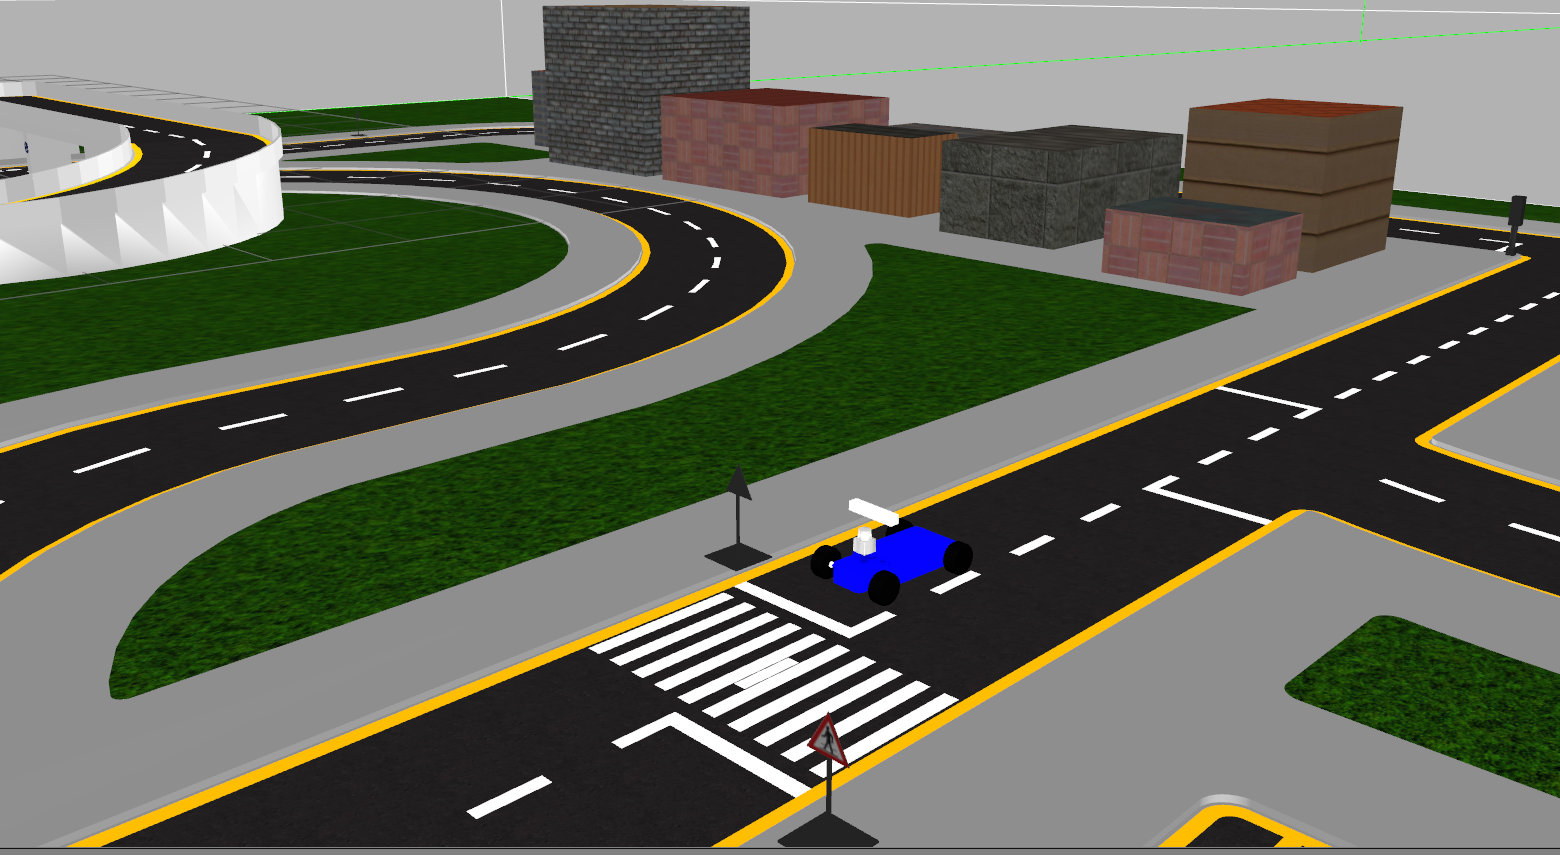
\includegraphics[width=\linewidth]{figures/simulation-environment2.png}
    \caption{}
  \end{subfigure}
  \caption{(a) Gazebo simulation environment top view. (b) The car, traffic
  signs, and the bridge in the simulation environment.}
  \label{figure:simulation-environment}
\end{figure}

Simulated sensors were also carefully tuned to reflect actual sensor behaviors,
but still actual camera images look blurrier. Moreover, we did not simulate the
changing lighting conditions and vibrations from the actuators. Figure
\ref{figure:camera-view} gives the actual and simulated camera views for
comparison.

\begin{figure}[h]
  \centering
  \begin{subfigure}[b]{0.4\linewidth}
      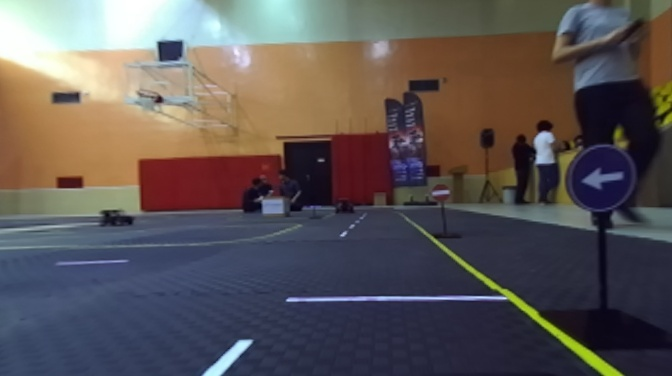
\includegraphics[width=\linewidth]{figures/actual-camera-view.jpg}
    \caption{}
  \end{subfigure}
  \begin{subfigure}[b]{0.4\linewidth}
      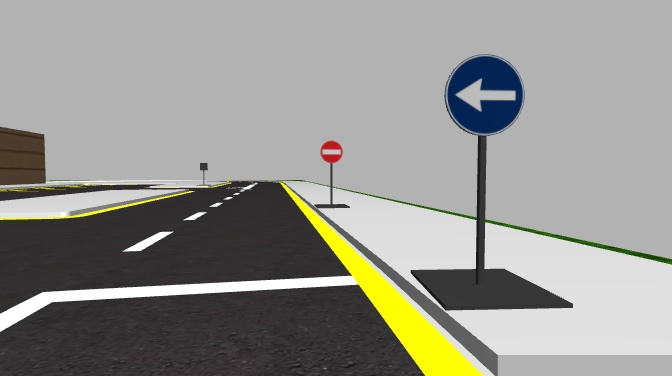
\includegraphics[width=\linewidth]{figures/simulated-camera-view.jpg}
    \caption{}
  \end{subfigure}
  \caption{(a) Actual camera view. (b) Simulated camera view.}
  \label{figure:camera-view}
\end{figure}

Despite all the peculiarities of the simulation environment, it made it
possible to quickly collect datasets without needing any additional hardware,
not even a joystick as it supports keyboard commands. We trained our
segmentation and classification models on those datasets and tested in the
simulation environment. We also developed our trajectory planning and control
algorithms in the simulation, which drastically reduced the risk of damaging
any equipment. On the whole, the simulation did not replace the real world, but
rather served as a flexible testbed.

\chapter{Scene Interpretation}
\label{chp:b4}

In this chapter, we present our mini driverless car's perception capabilities
and how it draws on these capabilities to interpret the current scene into
high-level driving behaviors by means of a rule-based system. We first discuss
our semantic segmentation model and semantic segmentation classes. Second, we
explain the methods we used to locate the right and left lanes with respect to
the body frame. Third, we describe our relatively small classification model
that runs on the top of the segmentation results to classify traffic signs and
lights. Then, we demonstrate our local maps that are used for locating nearby
obstacles. Finally, we introduce our behavior planner, which relates the given
the environmental perception with the traffic rules and picks a primitive
driving pattern accordingly.

\section{Environmental Perception}

\subsection{Semantic Segmentation}

Semantic segmentation is the backbone of our visual perception component. We
deploy a semantic segmentation deep learning model for which we manually
annotate each camera image into ego lane, right lane, left lane, roadside and
traffic sign classes using an image annotation tool, labelme
\cite{Ketaro2016LM}. Once trained, the segmentation model classifies each pixel
of the input image into these classes. In order to visualize the labels, we
assign a color for each class.  Figure \ref{figure:label-visualization}
illustrates segmentation labels blended on the camera images. We annotate
traffic lights and traffic signs with green, ego lane with blue, left lane with
yellow, right lane with red, roadside with pink and all other pixels are
considered background and assigned to black color.

\begin{figure}[h]
  \centering
  \begin{subfigure}[b]{0.4\linewidth}
    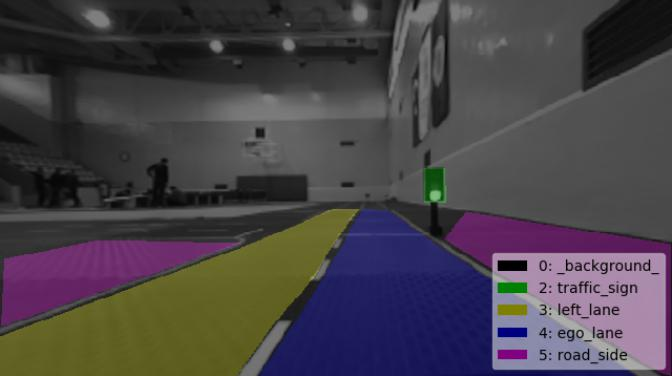
\includegraphics[width=\linewidth]{figures/label-visualization1.jpg}
    \caption{}
  \end{subfigure}
  \begin{subfigure}[b]{0.4\linewidth}
    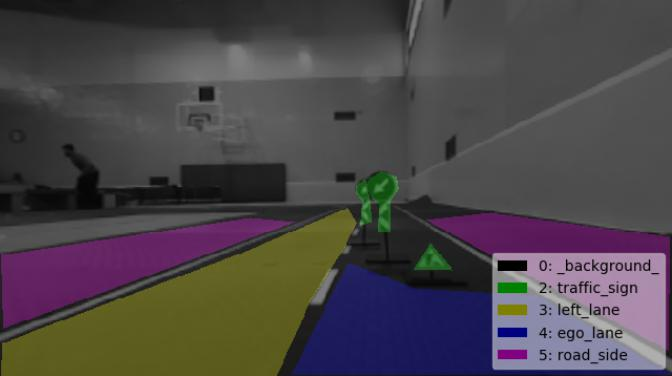
\includegraphics[width=\linewidth]{figures/label-visualization2.jpg}
    \caption{}
  \end{subfigure}
  \begin{subfigure}[b]{0.4\linewidth}
    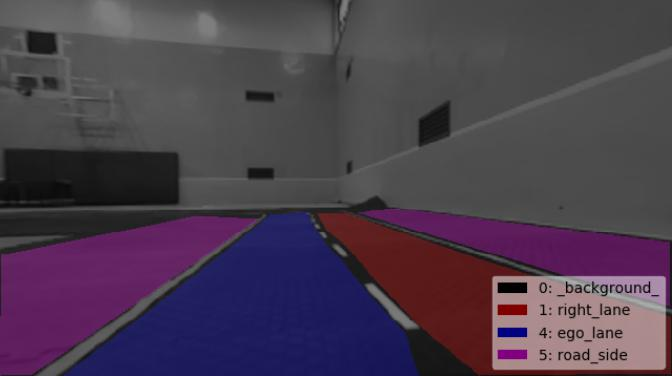
\includegraphics[width=\linewidth]{figures/label-visualization3.jpg}
    \caption{}
  \end{subfigure}
  \begin{subfigure}[b]{0.4\linewidth}
    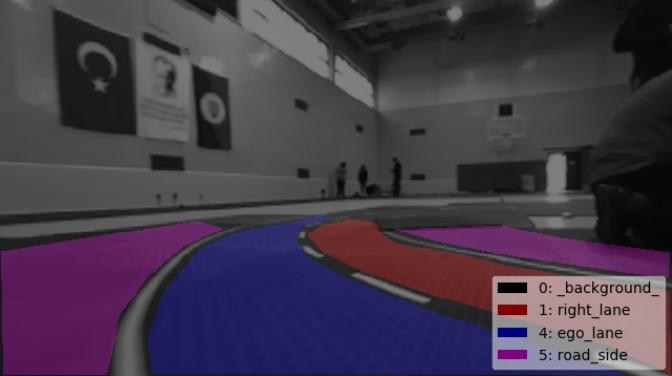
\includegraphics[width=\linewidth]{figures/label-visualization4.jpg}
    \caption{}
  \end{subfigure}
  \caption{(a) Traffic light, ego lane, left lane, and roadside labels. (b)
    Traffic signs, ego lane, left lane, and roadside labels. (c) Ego lane, right
    lane, and roadside labels. (d) Labels on a curvy road segment.}
  \label{figure:label-visualization}
\end{figure}

We adopt U-net architecture for our traffic scene segmentation task inspired
from \cite{Srihari2018SS}. U-net works well with a few training images and
yields fast and precise segmentations \cite{Ronneberger2015UNetCN}. As shown in
Figure \ref{figure:unet-architecture}, the U-net architecture is in shape of U,
thus the name U-net. Our slightly modified architecture inputs an RGB image of
size 128x128x3 and encodes it in the contraction side through applying multiple
blocks of layers. Each block takes an input and applies two 3x3 convolutions,
each followed by a batch normalization, ReLU activation, and a 2x2 max pooling
with stride 2 for downsampling. After each downsampling step, we double the
number of feature maps (i.e., the number of filters or channels).  Expansive
side decodes the captured features in the bottleneck section and also is made
of multiple blocks. Each expansive block applies a 2x2 up-convolution for
upsampling, halves the number of feature maps, concatenates the corresponding
feature maps from contracting and expansive sides, and finally applies two 3x3
convolutions, each followed by a batch normalization and ReLU activation. At
the output layer, we use a 1x1 convolution followed by a batch normalization
and softmax to map the resulting 16 feature maps to the desired number of
classes, which is 6 in our case including the background class.

\begin{figure}[h]
  \centering
  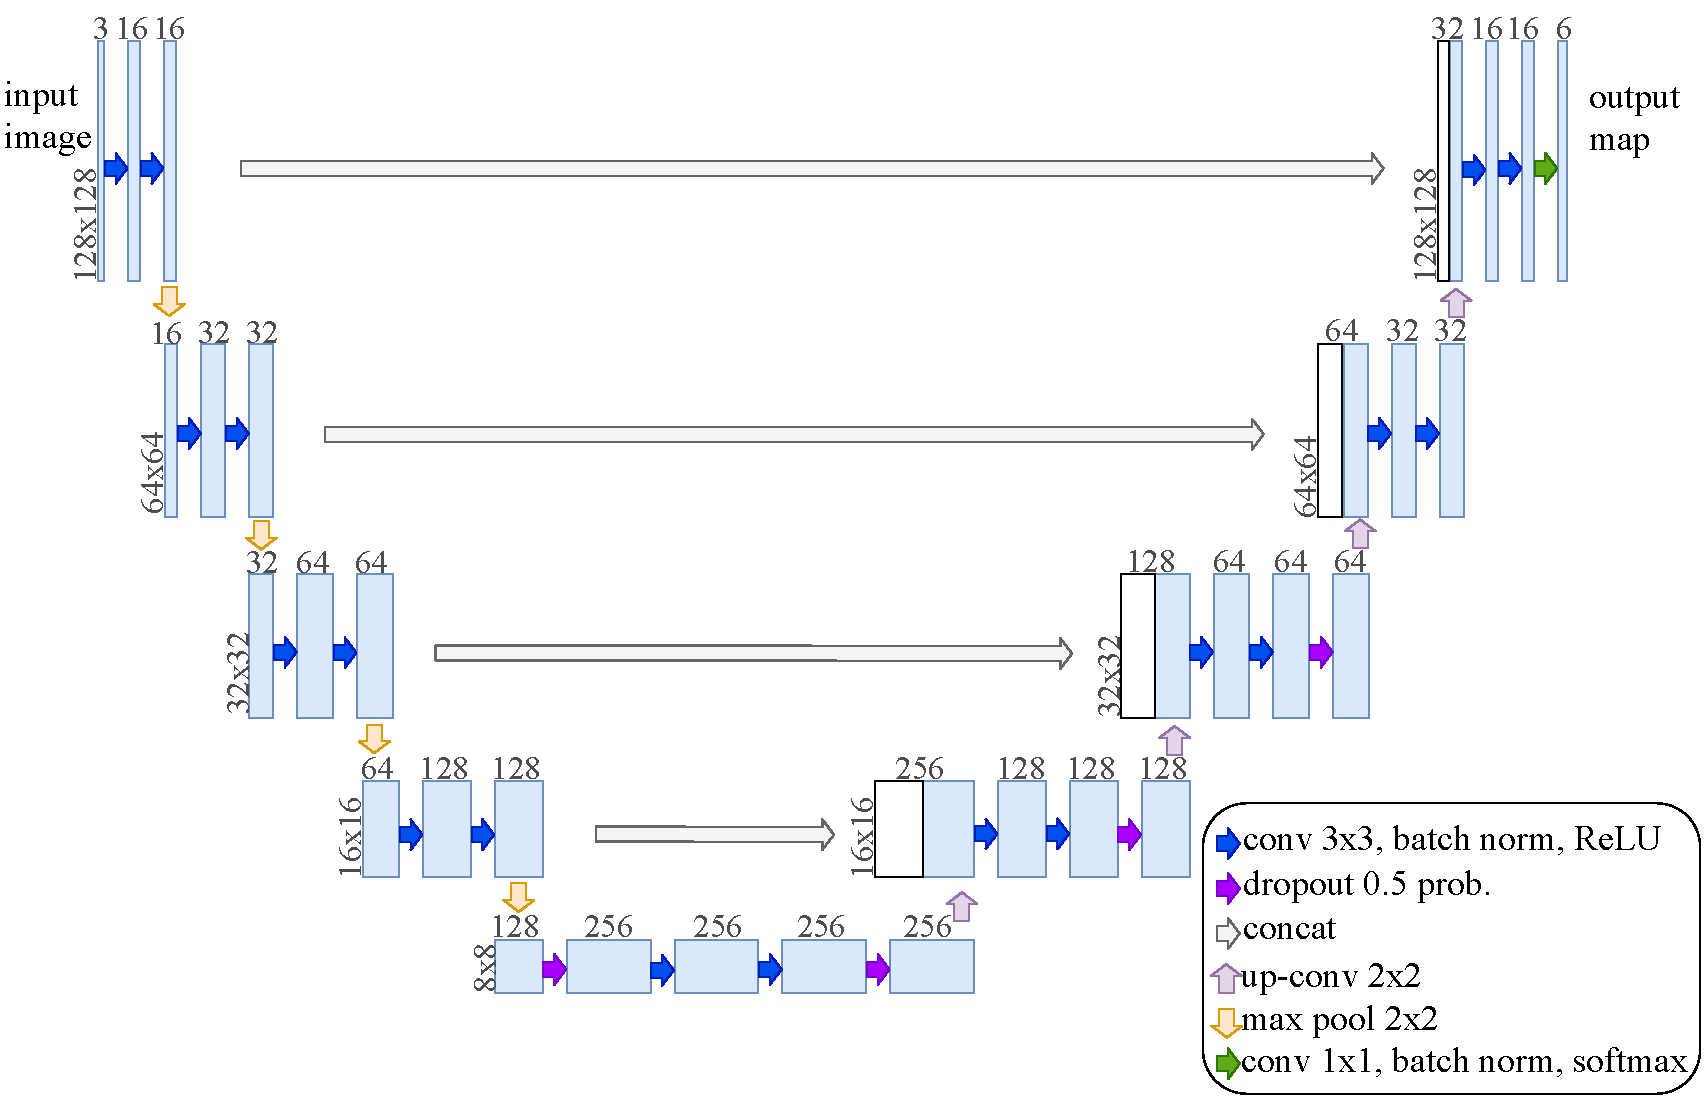
\includegraphics[width=1.0\textwidth]{figures/unet-architecture.pdf}
  \caption{Modified U-net architecture for semantic segmentation. Each blue box
    corresponds to a multi-channel feature map. The number of channels is
    given on the top of each box. The width x height sizes are provided at the
    lower left edge of each block of layers. White boxes denote the
    concatenated feature maps from the contracting side. The arrows denote
    different operations.}
  \label{figure:unet-architecture}
\end{figure}

In order to meet smooth driving experience requirements, the segmentation
inference shall run at 10 Hz and share the limited resources on the central
computer, which sets an upper bound for the size of our segmentation model.
Therefore, we resize down the camera images from 672x376 to 128x128. We also
lower the initial number of filters to 16, which is 64 in the original U-net
paper. Note that as opposed to the original architecture, we use paddings for
the convolutional layers so that the output of a convolution layer has the same
width and height as the input. As a result, we don't crop contracting feature
maps before concatenating them with the corresponding feature maps on the
expanding side. Another deviation from the original architecture is that we
train the model in batches(batch size of 8), so we apply batch normalization
following each 3x3 and 1x1 convolutional layers. We also place additional
dropout layers to the bottleneck section and expansive side. We use Adam
optimizer with sparse categorical cross entropy loss function from Keras which
ships with TensorFlow as a high-level API \cite{Abadi2015TF, Chollet2015Keras}.

\subsection{Lane Detection}

Because we are trying to navigate without a prior map of the environment as in
\cite{Meyer2018DeepSL}, the lane detection is used not only for adhering to the
traffic rules, but also for the whole navigation task until the car encounters
a traffic sign to change direction.

Our strategy for the lane detection is based on the semantic segmentation. We
first run an argmax on the output segmentation map across the channel axis and
assign a color to each channel as shown in Figure
\ref{figure:label-visualization}. Then we apply inverse perspective mapping to
obtain birdseye view as in Figure \ref{figure:inverse-perspective-mapping}.
The corners of the quadrilaterals in Figure
\ref{figure:inverse-perspective-mapping} are selected such that each pixel in
the birdseye view represents a 1x1 $cm^2$ in the world. Finally, we create a
point cloud from the birdeye view by downsampling it by a factor of 2 for
faster second order polynomial fitting to the lanes. The resultant birdseye
point cloud is also given in Figure \ref{figure:inverse-perspective-mapping}.

\begin{figure}[h]
  \centering
  \begin{subfigure}[b]{0.32\linewidth}
    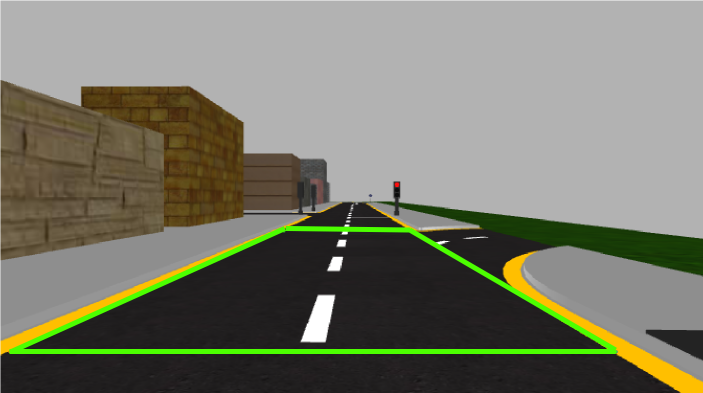
\includegraphics[width=\linewidth]{figures/before-ipm.png}
    \caption{}
  \end{subfigure}
  \begin{subfigure}[b]{0.32\linewidth}
    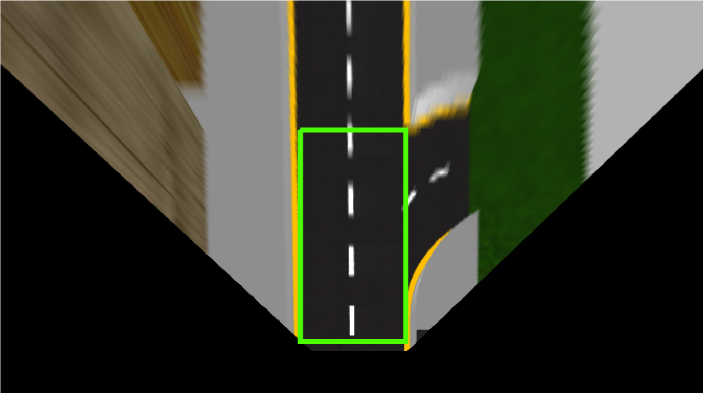
\includegraphics[width=\linewidth]{figures/after-ipm.png}
    \caption{}
  \end{subfigure}
  \begin{subfigure}[b]{0.32\linewidth}
    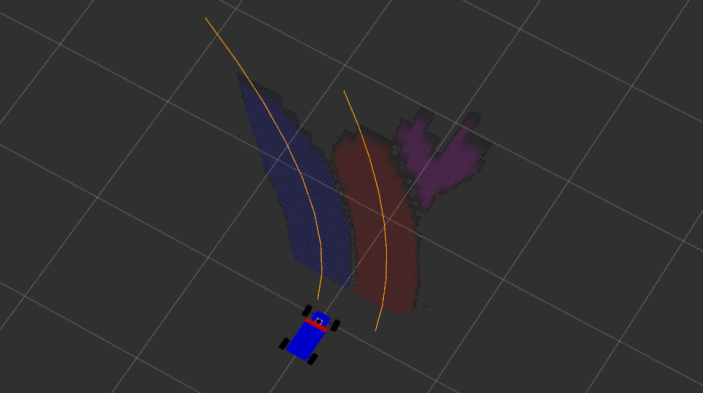
\includegraphics[width=\linewidth]{figures/birdseye-point-cloud.png}
    \caption{}
  \end{subfigure}
  \caption{(a) Before inverse perspective mapping. (b) Birdseye view after
    inverse perspective mapping. (c) Birdseye view point cloud with ego and
    left lane curves in orange.}
    \label{figure:inverse-perspective-mapping}
\end{figure}

In order to find midpoints along the lanes and make it more robust to erroneous
segmentation patches, we apply sliding window and guided searches for each
lane. Both search types are illustrated in Figure \ref{figure:lane-searches}
for the ego lane. It is straightforward to apply the same procedure for the
right and left lanes. While the sliding window search uses histogram to find
starting lane locations, guided search relies on the previous polynomial fits
with some margin. Every time we lose a lane, we initiate a sliding window
search for that particular lane. Once the lane is found, we switch to the
guided search as it is computationally less demanding. For each lane, we
average the coefficients of up to last 5 polynomial fits and obtain the
linearly spaced 9 points along the average polynomial curve. These 9 midpoints
for each lane are the waypoints that describe the lanes on the road.

\begin{figure}[h]
  \centering
  \begin{subfigure}[b]{0.32\linewidth}
    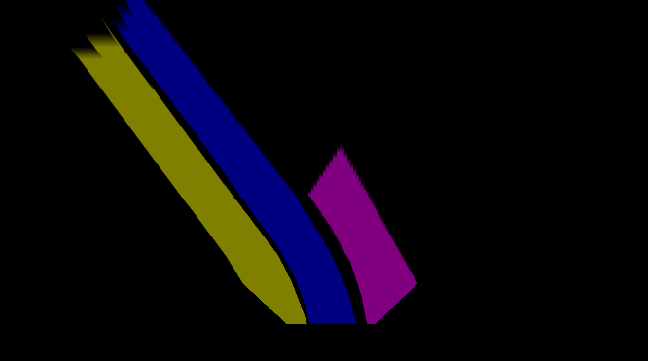
\includegraphics[width=\linewidth]{figures/segmentation-birdseye-view.png}
    \caption{}
  \end{subfigure}
  \begin{subfigure}[b]{0.32\linewidth}
    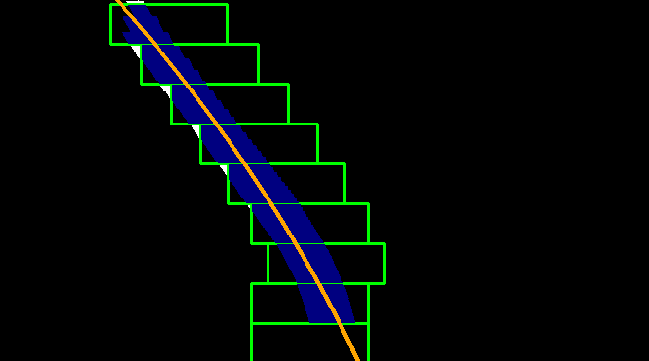
\includegraphics[width=\linewidth]{figures/sliding-window-search.png}
    \caption{}
  \end{subfigure}
  \begin{subfigure}[b]{0.32\linewidth}
    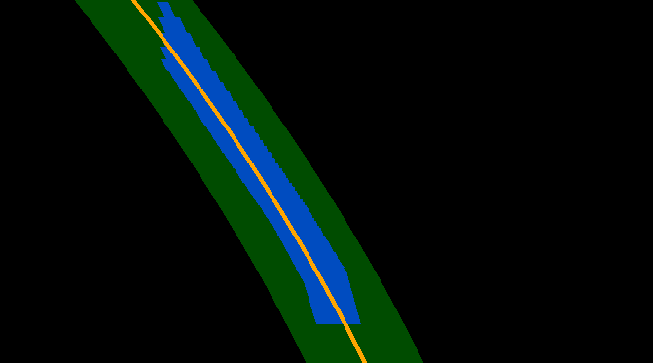
\includegraphics[width=\linewidth]{figures/guided-search.png}
    \caption{}
  \end{subfigure}
  \caption{(a) Segmentation birdseye view image. (b) Sliding window search for
    the ego lane. (c) Guided search for the ego lane on the next image frame
    after the the sliding window search. The green color denotes the sliding
    windows and guided search area. The orange color denotes the averaged
    polynomial curve.}
  \label{figure:lane-searches}
\end{figure}

\subsection{Sign Detection}

Traffic signs and lights regulate the car's behavior on certain conditions and
ensure the car travel the entire course with appropriate direction indications.
We treat the traffic lights the same way as the traffic signs, so the methods
used for the traffic signs also apply to the traffic lights.

Though there exist multiple well-established object detection deep learning
architectures with different size, performance and accuracy trade-offs
\cite{Gupta2019PerformanceCO, Rezatofighi2019GeneralizedIO}, our limited
resources in memory and computational power as well as the soft realtime
requirements at 10 Hz challenge us to use a more resource-friendly approach.
Instead of running an object detection model, we run a much simpler classifier
model on the segmented traffic sign patches. This approach also saves us from
labelling the whole dataset for the object detection in addition to the
semantic segmentation annotations. On the downside, we can not detect the signs
in an end-to-end fasion without resorting to computer vision techiques for
finding bounding rectangles for each sign patch in the segmentation output
\cite{Bradski2000CV}.

We first create a classification dataset selecting applicable signs from
existing datasets \cite{Timofte2009MultiviewTS, Stallkamp2012ManVC}. Because
these are small image patches irrespective of the scene, they worked well for
our miniature world. Having trained the classifier with existing datasets, we
run the classifier model along with the segmentation on our training courses,
which contain more traffic signs than usual. Then, we semi-automatically create
a new classification dataset by cropping and saving the classified traffic sign
patches. We later manually go through the saved image patches and ensure they
are in the correct class folder. Whenever an inappropriate image patch is
mistakenly classified as a traffic sign, we also put them into a special
negative class folder.  Augmentating our classification dataset in this manner
siginificantly improves our classifier as it learns from its own mistakes.

We classify \textit{PedestrianCrossing}, \textit{KeepLeft}, \textit{LooseGravel},
\textit{NoEntry}, \textit{Parking}, \textit{ParkingSlot}, \textit{RoadWork},
\textit{StraightOrRight}, \textit{TrafficLightGreen}, \textit{TrafficLightRed},
\textit{TurnLeft}, and \textit{Negative} classes. Figure
\ref{figure:traffic-sign-classes} illustrates these classes with image patches
automatically cropped from the training courses. The paches are converted to
grayscale and resized to 32x32 before fed into the classification model. The
classification architecture is depicted in Figure
\ref{figure:classification-architecture}. We train the model using Adam
optimizer with cross entropy loss in 32 batches applying shift, rescale, shear,
zoom, and brightness augmentation methods from Keras during
training\cite{Abadi2015TF, Chollet2015Keras}. Algorithm
\ref{algorithm:classification} explains the overall classification process on a
traffic sign segmentation mask.

\begin{figure}[h]
  \centering
  \begin{subfigure}[b]{0.15\linewidth}
    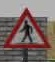
\includegraphics[width=\linewidth]{figures/signs/PedestrianCrossing.jpg}
    \caption{}
  \end{subfigure}
  \begin{subfigure}[b]{0.15\linewidth}
    
\includegraphics[width=\linewidth]{figures/signs/KeepLeft.jpg}
    \caption{}
  \end{subfigure}
  \begin{subfigure}[b]{0.15\linewidth}
    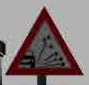
\includegraphics[width=\linewidth]{figures/signs/LooseGravel.jpg}
    \caption{}
  \end{subfigure}
  \begin{subfigure}[b]{0.15\linewidth}
    
\includegraphics[width=\linewidth]{figures/signs/NoEntry.jpg}
    \caption{}
  \end{subfigure}
  \begin{subfigure}[b]{0.15\linewidth}
    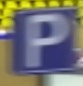
\includegraphics[width=\linewidth]{figures/signs/Parking.jpg}
    \caption{}
  \end{subfigure}
  \begin{subfigure}[b]{0.15\linewidth}
    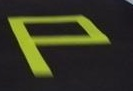
\includegraphics[width=\linewidth]{figures/signs/ParkingSlot.jpg}
    \caption{}
  \end{subfigure}
  \begin{subfigure}[b]{0.15\linewidth}
    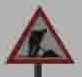
\includegraphics[width=\linewidth]{figures/signs/RoadWork.jpg}
    \caption{}
  \end{subfigure}
  \begin{subfigure}[b]{0.15\linewidth}
    
\includegraphics[width=\linewidth]{figures/signs/StraightOrRight.jpg}
    \caption{}
  \end{subfigure}
  \begin{subfigure}[b]{0.15\linewidth}
    
\includegraphics[width=\linewidth]{figures/signs/TrafficLightGreen.jpg}
    \caption{}
  \end{subfigure}
  \begin{subfigure}[b]{0.15\linewidth}
    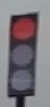
\includegraphics[width=\linewidth]{figures/signs/TrafficLightRed.jpg}
    \caption{}
  \end{subfigure}
  \begin{subfigure}[b]{0.15\linewidth}
    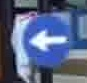
\includegraphics[width=\linewidth]{figures/signs/TurnLeft.jpg}
    \caption{}
  \end{subfigure}
  \begin{subfigure}[b]{0.15\linewidth}
    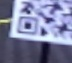
\includegraphics[width=\linewidth]{figures/signs/Negative.jpg}
    \caption{}
  \end{subfigure}
  \caption{Classified and saved traffic sign images from real and simulation
    training courses. (a) PedestrianCrossing, (b) KeepLeft, (c) LooseGravel, (d)
    NoEntry, (e) Parking, (f) ParkingSlot, (g) RoadWork, (h) StraightOrRight,
    (i) TrafficLightGreen, (j) TrafficLightRed, (k) TurnLeft, and (l)
    Negative.} \label{figure:traffic-sign-classes}
\end{figure}

\begin{figure}[h]
  \centering
  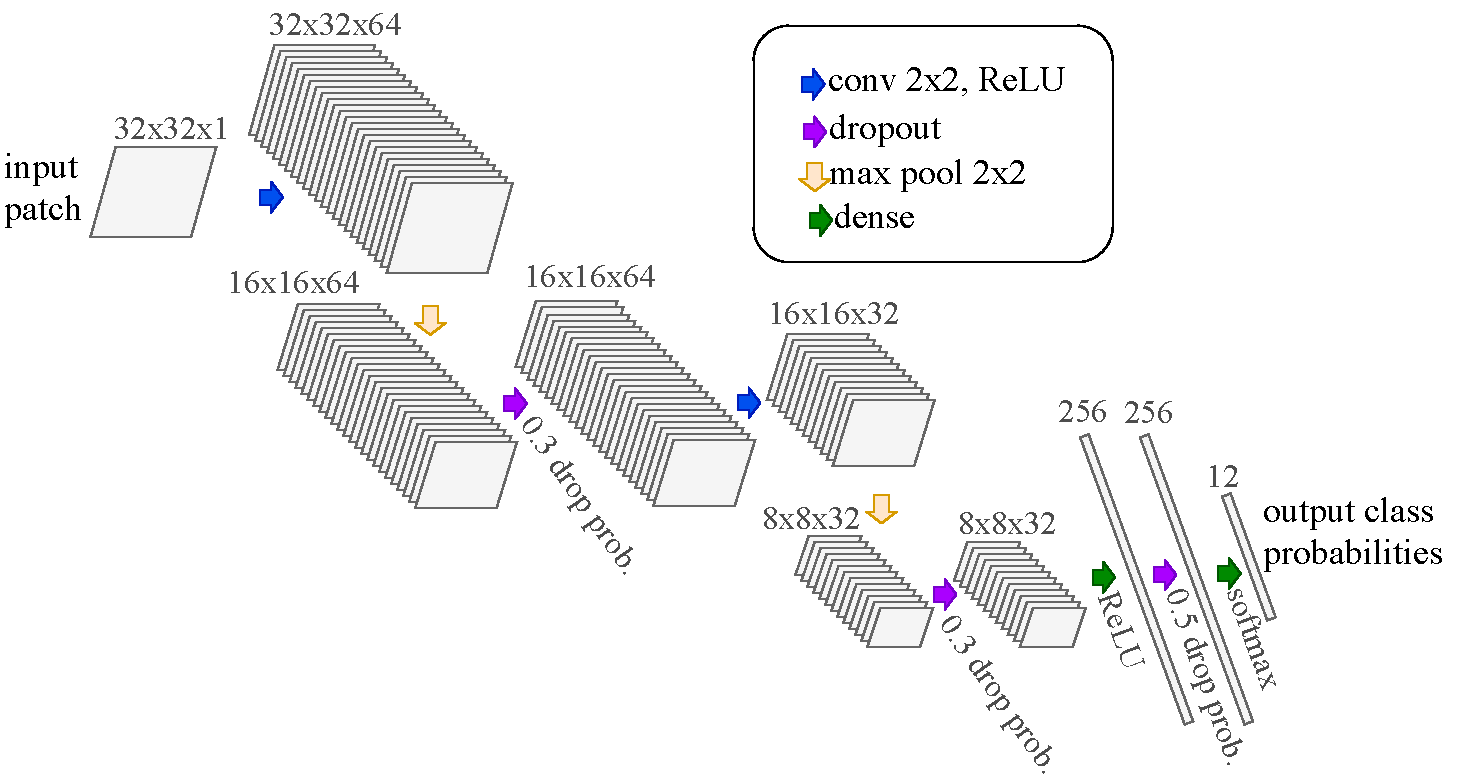
\includegraphics[width=.9\textwidth]{figures/classification-architecture.pdf}
  \caption{Classification architecture. $width \times height\times channel$ is
  given on each layer.}
  \label{figure:classification-architecture}
\end{figure}

\begin{algorithm}[h]
  \caption{Classification of segmented traffic signs.}
  \label{algorithm:classification}
  \begin{algorithmic}[1]
    \Procedure{PARSE-TRAFFIC-SIGNS}{$mask,rgb,depth,intrinsic,record,classes$}
    \State $cx, cy, fx, fy \gets intrinsic$
    \Comment{Unpack camera intrinsic parameters}
    \State $rects \gets list()$
    \State $k \gets 8$
    \Comment{Some pixel margin to the sign patch}
    \State $contours \gets cv2.findContours(mask)$
    \Comment{Use OpenCV to get traffic sign contours}
    \For{$contour$ \textbf{in} $contours$}
      \State $rect \gets cv2.boundingRect(contour)$
      \Comment{Use OpenCV to get a bounding rectangle of each contour}
      \If{$distance(rect, rects[i]) < 32$}
        \State $rects[i] \gets merge(rect, rects[i])$
        \Comment{Merge rectangles if they are too close}
      \EndIf
      \State $rects.append(rect)$
    \EndFor

    \State $t \gets currentTime()$
    \For{$class$ \textbf{in} $classes$}
      \State $events[class] \gets \textbf{False}$
      \If{$t - last(tracks[class]).t > 2$}
        \State \textbf{del} $tracks[class]$
        \Comment{Remove more than 2 second old tracks}
      \EndIf
    \EndFor
      \algstore{classification}
  \end{algorithmic}
\end{algorithm}

\begin{algorithm}
\ContinuedFloat
\caption{Classification of segmented traffic signs (continued)}
  \begin{algorithmic}
    \algrestore{classification}
    \For{$u,v,w,h$ \textbf{in} $rects$}
      \State $sign \gets rgb[v-k:v+h+k, u-k:u+w+k]$
      \State $class, confidance \gets classify(sign)$
      \Comment{Run inference}
      \If{$confidance > 0.8$}
        \State $z \gets mean(depth[v:v+h, u:u+w])$
        \State $x \gets z\frac{u-c_x}{f_x}$
        \State $y \gets z\frac{v-c_y}{f_y}$
        \State $tracks[class].append(x, y, z, t)$
        \If{$len(tracks[class]) > 3$ \textbf{and} $last(tracks[class]).x < 2.$}
          \Comment{We see the sign more than 3 times with enough confidance within
          a range of 2 meters, so we can safely report that we are tracking it}
          \State $objects[class] \gets (x, y, z, t)$
          \State $events[class] \gets \textbf{True}$
          \If{record \textbf{is True}}
            \State $name \gets unique()$
            \State $save(sign, class, name)$
            \Comment{Record the sign to further enrich the dataset}
          \EndIf
        \EndIf
      \EndIf
    \EndFor
    \State \textbf{return} $tracks, objects, events$
    \EndProcedure
  \end{algorithmic}
\end{algorithm}

\subsection{Obstacle Detection}

We maintain two different local occupancy grids in size and resolution in the
perception component. Each occupancy grid is driven by the same laser scan
message. While 3x3 grid with 0.1 meter/cell resolution is passed to the
trajectory planner, 4x4 grid with 0.2 meter/cell resolution is used to analyze
obstacle in the neighborhood that could change the current driving behavior
such as speed profile, which is also a parameter to the trajectory planner.
Figure \ref{figure:costmaps} demonstrates the local occupancy grids in action.
The car is always centered on the grids; therefore, the grids also move as the
car moves.

\begin{figure}[h]
  \centering
  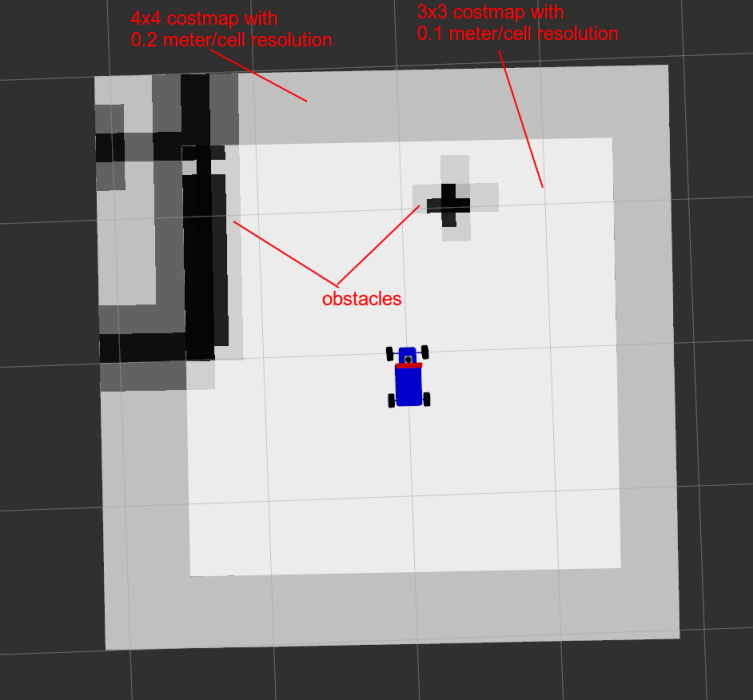
\includegraphics[width=.8\textwidth]{figures/costmaps.png}
  \caption{The small and large local occupancy grids.}
  \label{figure:costmaps}
\end{figure}

We generate two events from the large occupancy grid. The first event,
\textit{ObstacleAhead} indicates there is an obstacle ahead of the car within a
range of 2 meters. The other event, \textit{DangerousObstacle} alerts that
there is an obstacle dangerously too close to the car within 0.7 meters.
Algorithm \ref{algorithm:obstacle-detection} gives the steps for generating
these events.

\begin{algorithm}[h]
  \caption{Obstacle events.}
  \label{algorithm:obstacle-detection}
  \begin{algorithmic}[1]
    \Require Pose $x,y,\theta$ extracted from the latest odometry message.
    $\theta$ is the yaw angle in radian.
    \Procedure{PARSE-OBSTACLES}{$grid,x,y,\theta$}
    \State $nonzeroy, nonzerox \gets nonzero(grid)$
    \Comment{Get nonzero cells (i.e., the obstacle cells)}
    \State $obstaclex \gets nonzerox * grid.resolution + grid.origin.x$
    \State $obstacley \gets nonzeroy * grid.resolution + grid.origin.y$
    \State $diffx, diffy \gets obstaclex - x, obstacley - y$
    \State $angles \gets arctan(\frac{diffy}{diffx})$
    \State $angles \gets rad2deg(\theta - angles)$
    \State $mask = (angles < 10.) \& (angles > -10)$
    \State $events[ObstacleAhead] \gets count\_nonzero(mask) > 0$
    \State $distances \gets \sqrt{diffx^2 + diffy^2}$
    \State $mask = (angles < 10.) \& (angles > -10) \& (distances < 0.7)$
    \State $events[DangerousObstacle] \gets count\_nonzero(mask) > 0$
    \State \textbf{return} $events$
    \EndProcedure
  \end{algorithmic}
\end{algorithm}

\section{Behavior Planning}

Behavior planner consumes the events generated from the perception component.
It transitions the car into appropriate states depending on the hierarchical
finite state machine given in Figure \ref{figure:hfsm} as the events arrive.
When the car is in WAIT state, if there is no obstacle ahead and red light is
not observed, transition 1 is executed and the car starts driving itself. While
the car is moving, if it observes a pedestrian crossing sign or a red light, it
performs transition 2 and starts waiting until transition 1 conditions are
satisfied. In DRIVE state, the default behavior is to follow the lanes at
normal speed, 0.7 m/s. When the car come across any of straight or turn right,
turn left, or park signs, it stops lane following by sourcing predefined
waypoints for these signs to the trajectory planner instead of the waypoints
extracted from the lanes. In the event that the last predefined waypoint is
reached or a manual intervention through a joystick for an emergency while
following a predefined path, runs transition 4 to put the car back into the
lane following state. If any of LooseGravel, KeepLeft, RoadWork or
DangerousObstacle events reported while driving at the normal speed, the car
goes into SLOW SPEED state through transition 5 and starts driving at 0.5 m/s.
When none of these events are reported, the car switches back to the NORMAL
SPEED state. Finally, when the car sees a parking slot sign on the ground, it
performs transition 7 into the PARK state, in which the car moves into the
parking slot and stops.

\begin{figure}[h]
\centering
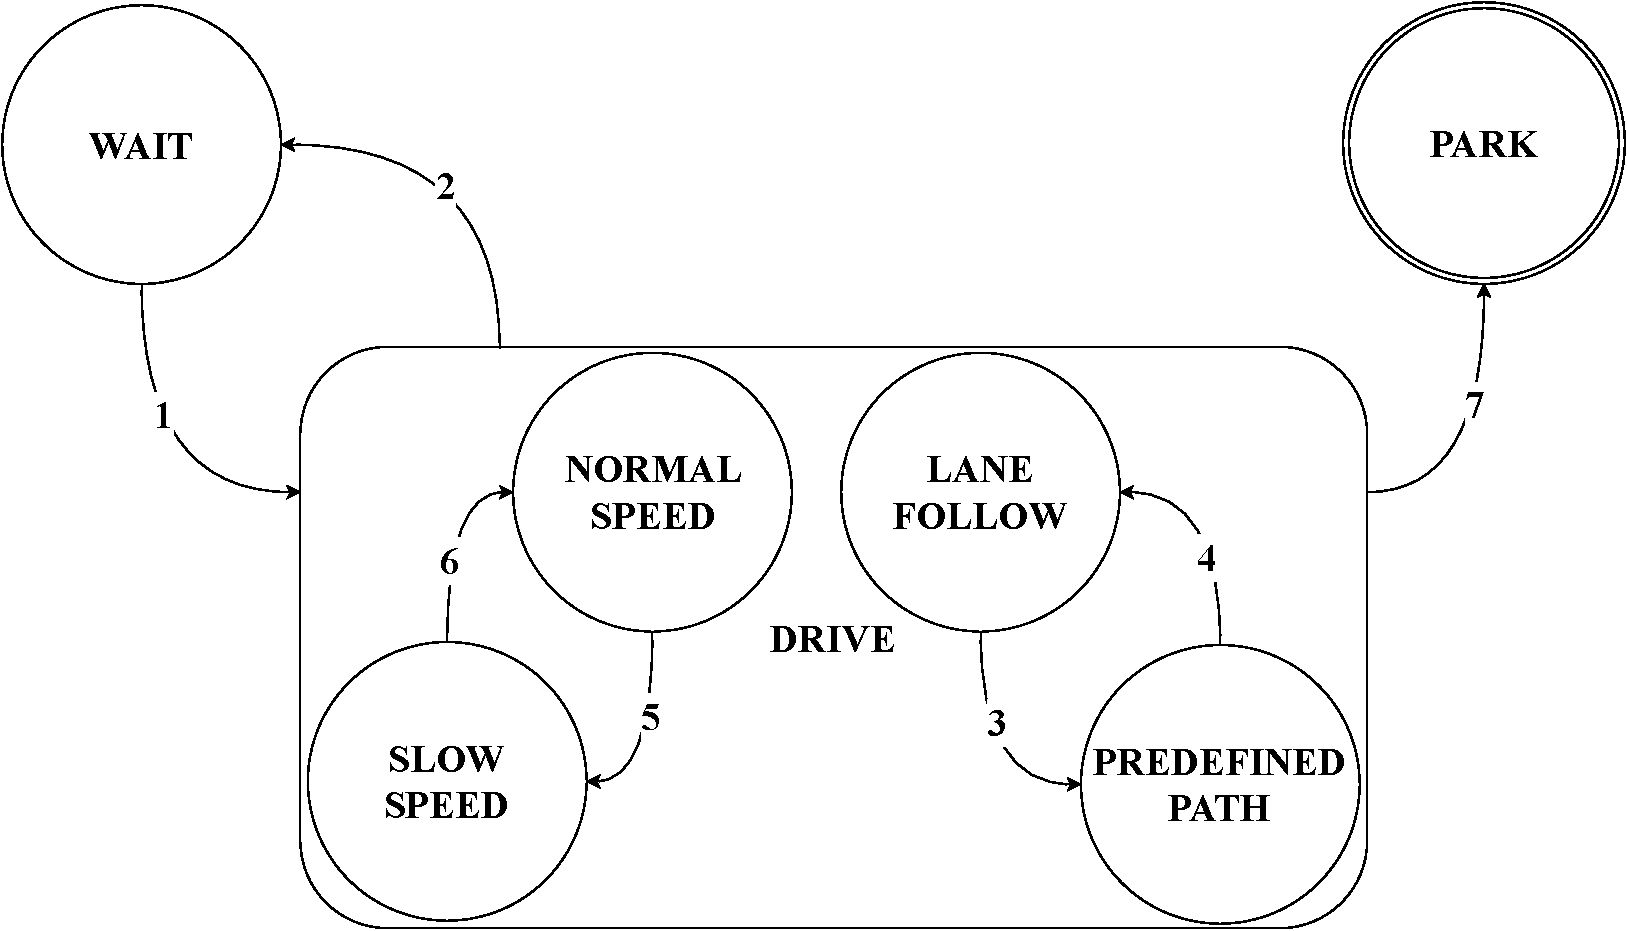
\includegraphics[width=.8\textwidth]{figures/hfsm.pdf}
\caption{Hierarchical finite state machine that governs the high-level behavior
of the car. The numbered arrows 1 to 7 denote the transitions between states.
DRIVE state has two sub-states to control speed profile and waypoint source to
the navigation module. PARK is the terminal state.}
\label{figure:hfsm}
\end{figure}

\chapter{Navigation}
\label{chp:b5}

In this chapter, we focus on our trajectory planning and control algorithms.
The trajectory planner receives a primitive behavior mode, for our case, either
stop or cruise mode, along with a set of waypoints as a reference path and
delivers a safe, feasible trajectory consisting of another set of waypoints
each has a recommended speed to the control block. The conrol block executes
the trajectory by adjusting the steering angle to closely follow the waypoints
at recommended speeds.

\section{Trajectory Planning}

We build a cubic spline curve from the reference waypoints to represent the
reference path. In order to generate trajectories along the reference path, we
use frenet frame as in \cite{cite14, cite15}. Because the map of the
environment is not known a priori for our scenario, the reference paths are
either extracted from the lanes or predefined for a specific traffic sign. We
define normal trajectory $d(t)$ and tangential trajectory $s(t)$ to our
reference path $\vec{r}(s)$ as shown in Figure \ref{figure:frenet}. To use the
same convention as \cite{cite15}, we also let $d(t)$ and $s(t)$ be offset
pattern and distance pattern, respectively. While the offset pattern
corresponds to lateral dispacement, distance pattern corresponds to
longitudinal acceleration and deceleration. We combine the two by
Equation \eqref{eq:trajectory} to obtain a trajectory.

\begin{figure}[h]
  \centering
  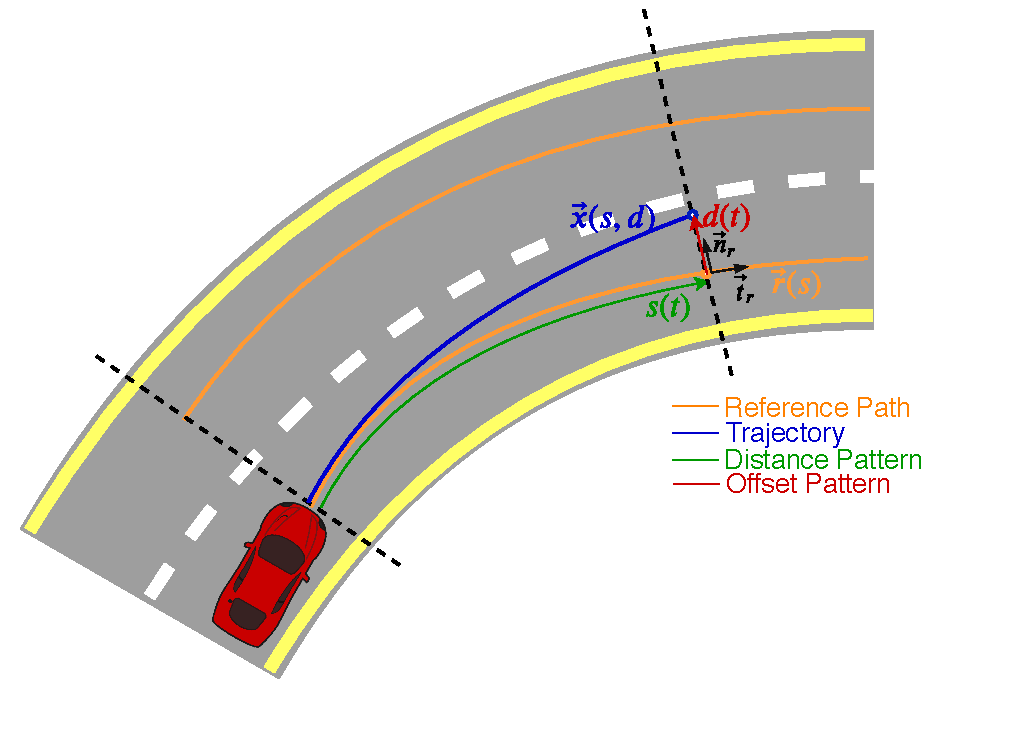
\includegraphics[width=1.0\textwidth]{figures/frenet-frame.pdf}
  \caption{Frenet frame based on the right reference path extracted
  from the right lane.}
  \label{figure:frenet}
\end{figure}

\begin{equation}
    \vec{x}(s(t), d(t)) = \vec{r}(s(t)) + d(t)\vec{n}_r(s(t))
\label{eq:trajectory}
\end{equation}

Offset and distance patterns are represented by 5-degree polynomials
in Equations \eqref{eq:dt} and \eqref{eq:st}.

\begin{equation}
    d(t) = a_0 + a_1t + a_2t^2 + a_3t^3 + a_4t^4 + a_5t^5
\label{eq:dt}
\end{equation}

\begin{equation}
    s(t) = a_0 + a_1t + a_2t^2 + a_3t^3 + a_4t^4 + a_5t^5
\label{eq:st}
\end{equation}

We generate a set of trajectories forward simulating various terminal
conditions for offset and distance patterns. $a_i$ and $b_i$ are calculated
using initial conditions $[d_0, \dot{d}_0, \ddot{d}_0]$, $[s_0, \dot{s}_0,
\ddot{s}_0]$ at $t_0$ and terminal conditions $[d_1, \dot{d}_1, \ddot{d}_1]$,
$[s_1, \dot{s}_1, \ddot{s}_1]$ at $t_1 = t_0 + \Delta T$, where $\Delta T$ is a
preview time in seconds. We use $4 < \Delta T < 6$ with $0.2$ second increments
for our offset and distance patterns. The offset pattern is defined as a
quintic function to control the lateral position.  The distance pattern is
defined using quartic and quintic function for cruise mode and stop mode,
respectively. In cruise mode, we don't pay attention to the terminal conditions
at longitudinal positions, but rather we focus on keeping the speed constant
around the speed profile set by the behavior planner; therefore, we set $b_5 =
0$. On the other hand, we specify a longitudinal position as a terminal
condition for the stop mode expecting the car to confortably slow down and
eventually stop at the specified position.

For the offset pattern, minimizing the lateral speed and accelaration leads to
a more confortable driving experience, so  we choose the terminal conditions
$[\Delta d, 0, 0]$ for the candidate trajectories, where $\Delta d = \{-0.1, 0,
1.0\}$ m. For cruise mode, we choose $[\dot{s}_1 + \Delta \dot{s}_1,
\ddot{s}_1]$, where $\Delta \dot{s}_1 = \{-0.1, 0, 0.1\}$ m/s and $\dot{s}_1$
is the target speed set by the behavior planner. For stop mode, we choose
$[s_1, 0, 0]$ terminal conditions, where $s_1$ is the stop position.

For all candidate trajectories, we apply a sanity check to see the candidate is
actually drivable. If there is an overlap between an obstacle grid of the
occupancy grid map and the car's bounding circle along a trajectory, we
conclude that the trajectory is not drivable. Non-drivable trajectories are
eliminated from the trajectory set. If no drivable trajectory is left, we set
the speed to zero until a valid trajectory is found again. Otherwise, the
trajectory with the minimum cost is selected among the surviving trajectories
as the best trajectory and forwarded to the controller for execution.
The cost function $C$ is defined in Equations \eqref{eq:cost1} -
\eqref{eq:cost3}.

\begin{equation}
    C = k_{path}C^i_{path} + k_dC_d + k_sC_s
\label{eq:cost1}
\end{equation}

\begin{equation}
    C_d = k_j\int_{t_0}^{t_1}\dddot{d}(t)dt + k_x\Delta T + k_y\Delta d^2
\label{eq:cost2}
\end{equation}

\begin{equation}
    C_s =
    \begin{cases}
        k_j\int_{t_0}^{t_1}\dddot{s}(t)dt + k_x\Delta T + k_y\Delta s^2,
        &\text{if stop mode;} \\
        k_j\int_{t_0}^{t_1}\dddot{s}(t)dt + k_x\Delta T + k_y\Delta \dot{s}^2,
        &\text{if cruise mode,}
    \end{cases}
\label{eq:cost3}
\end{equation}

where $C_d$ and $C_s$ are the costs from offset and distance patterns,
respectively. Both terms include integral of jerks, preview times, and
dispacement of terminal conditions. In multi-lane settings, $C^i_{path}$ is the
lane cost for \textit{i}th lane. For our scenario, we have only two lanes;
therefore, we assign a higher cost to the left lane so as to prevent the car
from occupying the left lane when the right lane is free as shown in Figure
\ref{figure:frenet-lanes}. In this way, the car automatically shifts to the
left lane when the right lane is blocked. Similarly, the car chooses the right
lane when it is available as it would be less costly than driving on the left
lane. We use $k_j = k_x = 0.1$ and $k_d = k_s = k_{path} = 1.0$ for our cost
evaluations.

\begin{figure}[h]
  \centering
  \begin{subfigure}[b]{1.0\linewidth}
      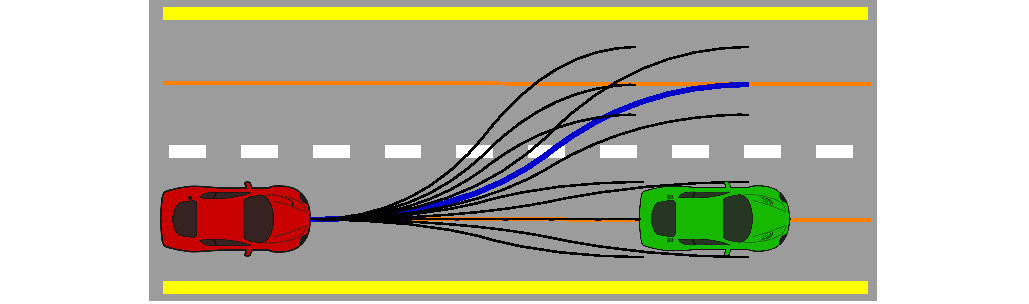
\includegraphics[width=\linewidth]{figures/frenet-shift-left-lane.pdf}
    \caption{}
  \end{subfigure}
  \begin{subfigure}[b]{1.0\linewidth}
      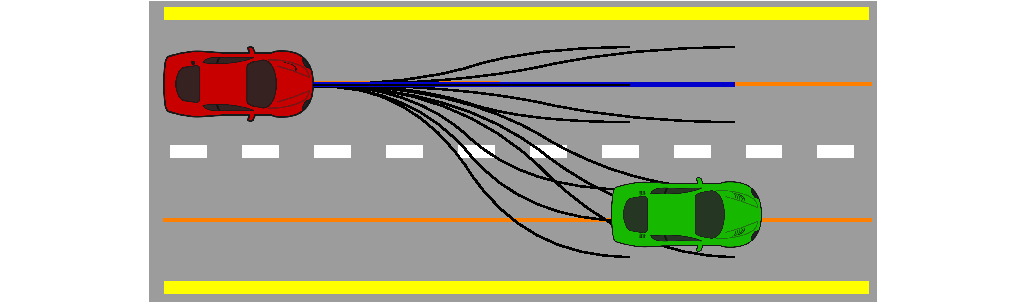
\includegraphics[width=\linewidth]{figures/frenet-keep-left-lane.pdf}
    \caption{}
  \end{subfigure}
  \begin{subfigure}[b]{1.0\linewidth}
      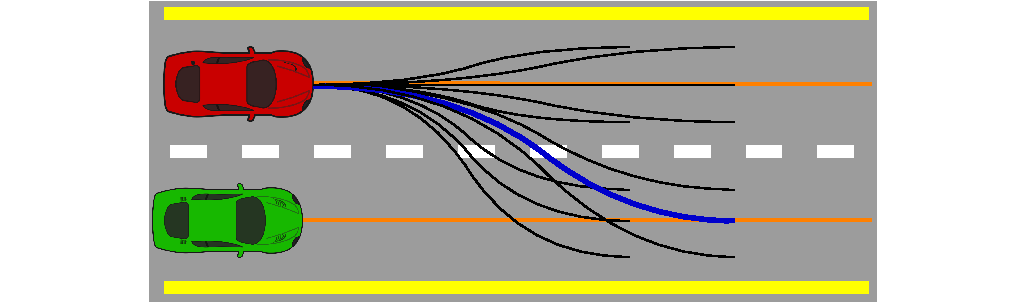
\includegraphics[width=\linewidth]{figures/frenet-shift-right-lane.pdf}
    \caption{}
  \end{subfigure}
  \caption{Example multi-lane driving scenario. The thick blue trajectory is
      the optimal trajectory for different cases. (a) The right lane is
      blocked, so the car attempts to change lane to the left for overtaking.
      (b) The right lane is still blocked, so the car keeps occupying the left
  lane. (c) Because the right lane is less costly when both lanes are
  available, the car shifts back to right lane.}
  \label{figure:frenet-lanes}
\end{figure}

\section{Trajectory Execution}

We use pure pursuit control algorithm to track the given optimal trajectory.
The algorithm relies on the nonholonomic constraints of the car. Let car
configuration be $\textbf{q} = [x y \theta]^T$, where $(x, y)$ is the position
and $\theta$ is the orientation of the car. Nonholonomic constraints satisfy
Equation \eqref{eq:nonholonomic}.

\begin{equation}
    \dot{x}\sin(\theta) - \dot{y}\cos(\theta) = 0
\label{eq:nonholonomic}
\end{equation}

such that longitudinal and lateral forces applied on the car tires are always
smaller than the maximum friction between the tires and the ground \cite{cite18}.
In other words we assume the car does not slip. With this constaints, we
estimate the steering angle in terms of turning radius $R$ and the wheelbase of
the car $L_b$ from Figure \ref{figure:steering} in Equation
\eqref{eq:steering}.

\begin{equation}
    \delta = \tan^{-1}(\frac{L_b}{R})
\label{eq:steering}
\end{equation}

\begin{figure}[h]
  \centering
  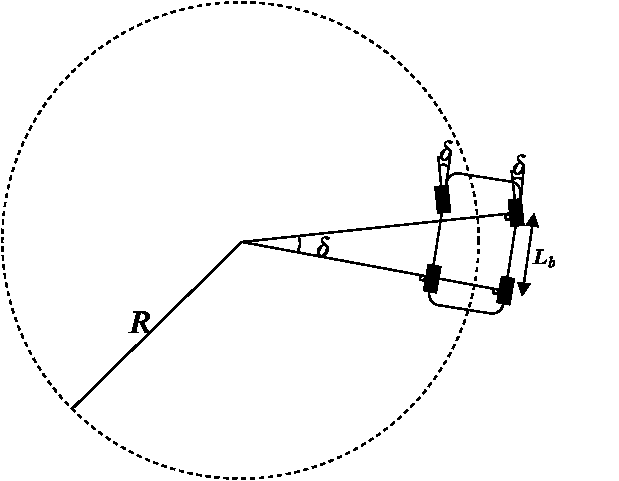
\includegraphics[width=0.8\textwidth]{figures/pure-pursuit-steering.pdf}
  \caption{Estimation of steering angle in terms of turning radius $R$ and
  wheelbase $L_b$.}
  \label{figure:steering}
\end{figure}

Given an optimal trajectory, we first find a point ahead of the car on the
trajectory such that the distance between the point and the car is the smallest
distance greater than a lookahead distance $L$. This is illustrated in Figure
\ref{figure:radius}.

\begin{figure}[h]
  \centering
  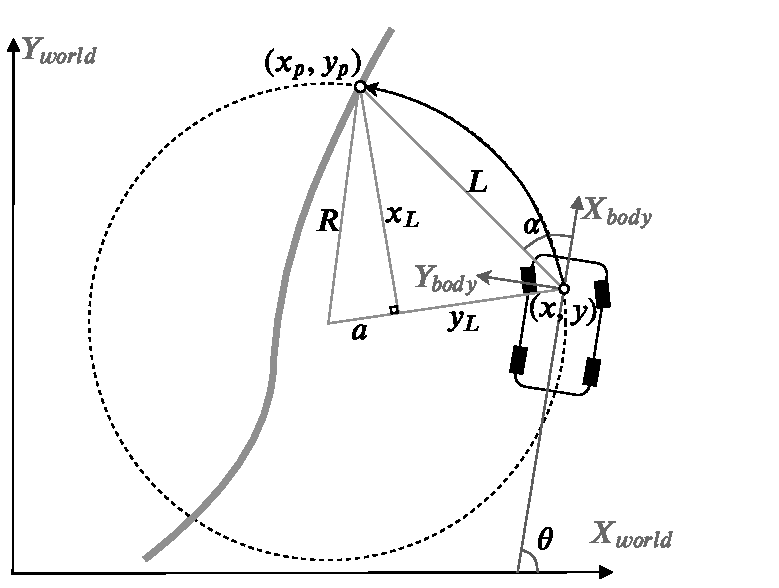
\includegraphics[width=0.8\textwidth]{figures/pure-pursuit-radius.pdf}
  \caption{Illustration of lookahead distance $L$ and feedback angle $\alpha$.}
  \label{figure:radius}
\end{figure}

From the figure, we write down the following equations:

\begin{equation}
    L^2 = x^2_L + y^2_L
\label{eq:radius1}
\end{equation}

\begin{equation}
    R^2 = a^2 + x^2_L
\label{eq:radius2}
\end{equation}

\begin{equation}
    R = a + y_L
\label{eq:radius3}
\end{equation}

\begin{equation}
    \sin{\alpha} = \frac{y_L}{L}
\label{eq:radius4}
\end{equation}

Combining \eqref{eq:radius1}, \eqref{eq:radius2}, and \eqref{eq:radius3}, we
obtain

\begin{equation}
    R = \frac{L^2}{2y_L}
\label{eq:radius5}
\end{equation}

Substituting \eqref{eq:radius4} in \eqref{eq:radius5}, we obtain and turning
radius $R$ in terms of feedback angle $\alpha$ and lookahead distance $L$.

\begin{equation}
    R = \frac{L}{2\sin{\alpha}}
\label{eq:radius6}
\end{equation}

Feedback angle $\alpha$ is computed by the car configuration $\textbf{q} = [x y
\theta]^T$ and the position of the lookahead point $(x_p, y_p)$ in the world
coordinates. Note that we take the midpoint of the front axle as the car
position in the world coordinates.

\begin{equation}
    \alpha = \tan^{-1}(\frac{y_p - y}{x_p - x}) - \theta
\label{eq:alpha}
\end{equation}

Finally, using \eqref{eq:steering} and \eqref{eq:radius6}, we derivate the
steering angle $\delta$ in terms of feedback angle $alpha$, constant wheelbase
$L_b$, and lookahead distance $L$.

\begin{equation}
    \delta = \tan^{-1}(\frac{2L_b\sin\alpha}{L})
\label{eq:delta}
\end{equation}

In order to tune the controller, we need to choose a lookahead distance $L$.
\cite{cite18} suggests $L = 2R_{min}$, where $R_{min} =
\frac{L_b}{\tan({\delta_{max})}}$. For our car, the max steering angle
$\delta_{max} = 0.34$ rads and the wheelbase $L_b = 0.25$ meters. Therefore, we
use $L = 1.4$. Figure \ref{figure:lookahead} illustrates the relation between
$R_{min}$ and $L$.


\begin{figure}[h]
  \centering
  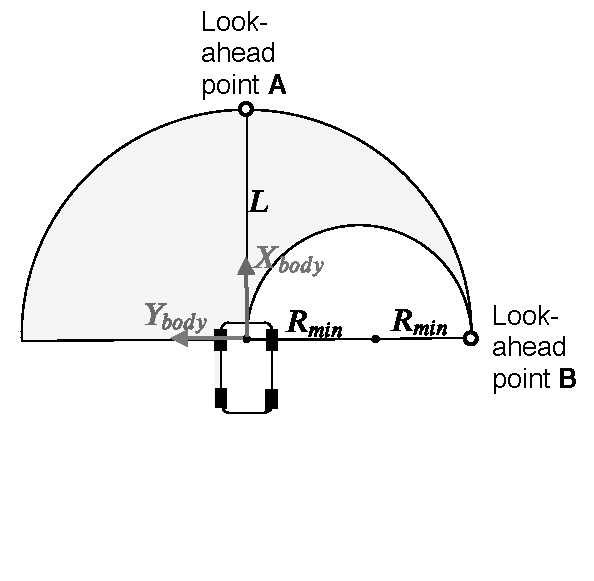
\includegraphics[width=0.8\textwidth]{figures/pure-pursuit-lookahead.pdf}
  \caption{Illustration of lookahead distance $L$ and minimum turning radius
  $R_{min}$ for tuning the pure pursuit controller.}
  \label{figure:lookahead}
\end{figure}

One problem with Equation \eqref{eq:delta} is that it does not account for the
speed. As the speed increases, steering angle $\delta$ becomes more sensitive
to the feedback angle $\alpha$ \cite{18}. WE address this problem by adding a
speed factor to lookahead distance $L$ in Equation \eqref{eq:lookahead}.

\begin{equation}
    L \leftarrow L + kv
\label{eq:lookahead}
\end{equation}

where $v$ is the recommended speed by the trajectory planner, $k$ is the look
forward gain. We use $k = 1$.

We compute a steering angle $\delta$ every time we receive an odometry message,
which is published at 15 Hz and contains the current car configuration
information.

\chapter{Experiments and Results}
\label{chp:b6}

We conducted various experiments for different scenarios in the simulation and
real miniature courses. In this chapter, we introduce our courses and datasets
collected from the courses. We evaluate our semantic segmentation and
classification deep learning models based on these datasets. We then demostrate
the behavior of our car on different traffic scenarios.

\section{Race Courses and Datasets}

Our experiments are based on four different courses. The first course is the
course provided by OpenZeka  two days before the competition, so it was not
available for use during the development. The second course is the one we
constructed in our laboratory, which is spatially no larger than the bridge
area of the actual competition course. We used it to collect simple images and
test our hardware setup to ensure the car is functioning properly. The third
one was developed in Gazebo simulation environment similar to the competition
course. We developed the fourth course in the simulation to semi-automatically
collect extra traffic sign images. Figure \ref{figure:annotated-courses}
illustrates the courses with semantic segmentation annotations.

\begin{figure}[h]
  \centering
  \begin{subfigure}[b]{0.4\linewidth}
    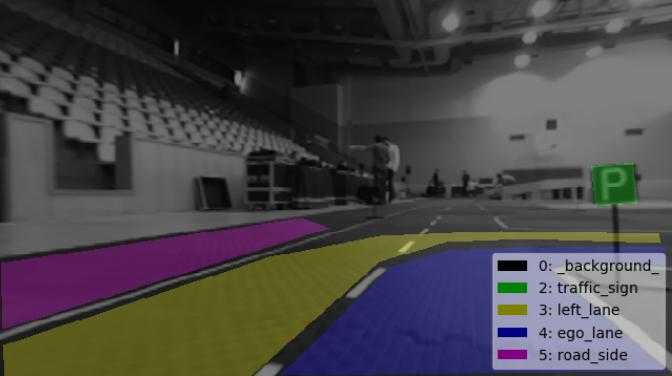
\includegraphics[width=\linewidth]{figures/course1.jpg}
    \caption{Course 1}
  \end{subfigure}
  \begin{subfigure}[b]{0.4\linewidth}
    \includegraphics[width=\linewidth]{figures/course2.jpg}
    \caption{Course 2}
  \end{subfigure}
  \begin{subfigure}[b]{0.4\linewidth}
    \includegraphics[width=\linewidth]{figures/course3.jpg}
    \caption{Course 3}
  \end{subfigure}
  \begin{subfigure}[b]{0.4\linewidth}
    \includegraphics[width=\linewidth]{figures/course4.jpg}
    \caption{Course 4}
  \end{subfigure}
  \caption[Real and simulated course scenes]{Example scenes from the courses.
    Course 1 is the official competition course. Course 2 is a small track
    constructed in the laboratory. Course 3 is a simulation of Course 1. Course
    4 is used to semi-automatically collect extra traffic sign images. It is
    not used for training or testing the semantic segmentation model.}
  \label{figure:annotated-courses}
\end{figure}

We split semantic segmentation dataset into training and testing sets as shown
in Table \ref{table:semantic-segmentation-dataset}. For classification dataset,
we started with a collection of relevant signs from existing datasets
\cite{Timofte2009MultiviewTS, Stallkamp2012ManVC, Shakhuro2016RussianTS,
Serna2018ClassificationOT, MaldonadoBascn2007RoadSignDA}. Then, we expand the
dataset by automatically cropping the sign patches from the images collected
from all our four courses as the car drives itself. The new sign patches are
manually arranged and merged into the existing classification dataset. Details
of the final classification dataset is presented in Table
\ref{table:classification-dataset}.

\begin{table}[h]
  \begin{center}
    \caption[Traffic scene semantic segmentation dataset]{Traffic scene
      semantic segmentation dataset.}
    \label{table:semantic-segmentation-dataset}
    \begin{tabular}{|c|c|c|}
      \hline
      \textbf{Course}   & \textbf{Training} & \textbf{Testing} \\
      Course 1          & 2249              & 212              \\
      Course 2          & 169               & 10               \\
      Course 3          & 230               & 29               \\
      \hline
      \textbf{Total}    & 2648              & 251              \\
      \hline
    \end{tabular}
  \end{center}
\end{table}


\begin{table}[h]
  \begin{center}
    \caption[Traffic sign classification dataset]{Traffic sign classification
      dataset.}
    \label{table:classification-dataset}
    \begin{tabular}{|c|c|c|c|}
      \hline
      \textbf{Class}     & \textbf{Training} & \textbf{Testing} & \textbf{Auto-cropped} \\
      \hline
      PedestrianCrossing & 704               & 89               & 470 \\
      KeepLeft           & 844               & 83               & 594 \\
      LooseGravel        & 533               & 60               & 593\\
      NoEntry            & 502               & 83               & 306 \\
      Parking            & 497               & 90               & 237 \\
      ParkingSlot        & 1730              & 60               & 1790 \\
      RoadWork           & 1741              & 86               & 237 \\
      StraightOrRight    & 1106              & 89               & 848 \\
      TrafficLightGreen  & 422               & 76               & 192 \\
      TrafficLightRed    & 1147              & 72               & 1095 \\
      TurnLeft           & 817               & 93               & 502 \\
      Negative           & 984               & 60               & 1044 \\
      \hline
      \textbf{Total}     & 11027             & 961              & 7908 \\
      \hline
    \end{tabular}
  \end{center}
\end{table}

\section{Perception Evaluation}

We evaluate our semantic segmentation model using IoU, Precision, Recall, and
F1 scores for each class given in Table
\ref{table:semantic-segmentation-test-results}. Despite the fact that we used
our own dataset, we compare our lane segmentation results to the results
reported by Barnes et al. \cite{Barnes2016FindYO} and Meyer et al.
\cite{Meyer2018DeepSL} as they are mostly relevant. For ego lane, which is the
main enabler for driving, Barnes et al. \cite{Barnes2016FindYO} achieve up to
85\% IoU and Meyer et al. \cite{Meyer2018DeepSL} achieve 80\% IoU. We achieved
88\% IoU on our dataset. However, note that our lanes are more obvious
compared to real traffic scenes. In real scenes, lane lines are often obscured
or worn-out. For the same reason, our results for neighboring lanes (i.e.,
right and left lanes) are better than the corresponding results presented by
Meyer et al. \cite{Meyer2018DeepSL} for opposite and parallel lanes. Our ego
lane precision, recall, and F1 scores are also comparable to the results
provided by these studies.

One can notice from Table \ref{table:semantic-segmentation-test-results} that
the right lane IoU is considerably smaller than that of the other lanes and
road side. This is because right lane is underrepresented in the dataset as we
most of the time drive the car on the right lane, effectively using it as the
ego lane. The same reason is also applicable for traffic signs. Traffic signs
are small, rare, and often located towards the edge of the images.

\begin{table}[h]
  \begin{center}
    \caption[Semantic segmentation test results]{Semantic segmentation
      test results.}
    \label{table:semantic-segmentation-test-results}
    \begin{tabular}{|c|c|c|c|c|}
      \hline
      \textbf{Class} & \textbf{IoU} & \textbf{Precision} & \textbf{Recall} & \textbf{F1}  \\
      Background     & 94.43\%      & 97.81\%            & 96.43\%         & 97.12\%      \\
      Ego Lane       & 88.48\%      & 92.29\%            & 93.18\%         & 92.73\%      \\
      Left Lane      & 83.52\%      & 87.83\%            & 94.49\%         & 91.04\%      \\
      Road Side      & 71.97\%      & 78.49\%            & 89.58\%         & 83.67\%      \\
      Right Lane     & 51.32\%      & 55.60\%            & 90.19\%         & 68.79\%      \\
      Traffic Sign   & 58.12\%      & 79.52\%            & 71.81\%         & 75.47\%      \\
      \hline
      \textbf{All}   & 74.64\%      & 81.92\%            & 89.28\%         & 84.80\%      \\
      \hline
    \end{tabular}
  \end{center}
\end{table}

For traffic sign detection, we run a classification model on top of the
semantic segmentation that proposes regions to the classification
network. Table \ref{table:classification-test-results} presents the detailed
performance metrics of our 97.45\% accurate classifier.

We find adding an extra negative class helpful to improve overall
classification performance. Nonetheless, \textit{Negative} class also has false
negatives lowering its recall as given in Table
\ref{table:classification-test-results}. In other words, a non-traffic sign
region can still be classified as a traffic sign as shown in Figure
\ref{figure:real-course-detection-bad}.

\begin{table}[h]
  \begin{center}
    \caption[Traffic sign classification test results]{Traffic sign
      classification test results.}
    \label{table:classification-test-results}
    \begin{tabular}{|c|c|c|c|}
      \hline
      \textbf{Class}     & \textbf{Precision} & \textbf{Recall}  & \textbf{F1-score} \\
      \hline
      KeepLeft           & 100.00\%           & 100.00\%         & 100.00\% \\
      LooseGravel        & 100.00\%           & 100.00\%         & 100.00\% \\
      NoEntry            & 95.40\%            & 100.00\%         &  97.65\% \\
      Parking            & 98.86\%            & 96.67\%          &  97.75\% \\
      ParkingSlot        & 84.51\%            & 100.00\%         &  91.60\% \\
      PedestrianCrossing & 97.72\%            & 69.63\%          &  97.17\% \\
      RoadWork           & 95.50\%            & 98.84\%          &  97.14\% \\
      StraightOrRight    & 100.00\%           & 97.75\%          &  98.86\% \\
      TrafficLightGreen  & 98.68\%            & 97.37\%          &  98.01\% \\
      TrafficLightRed    & 100.00\%           & 97.22\%          &  98.60\% \\
      TurnLeft           & 98.91\%            & 97.85\%          &  98.37\% \\
      Negative           & 100.00\%           & 85.00\%          &  91.90\% \\
      \hline
    \end{tabular}
  \end{center}
\end{table}

In order to evaluate our traffic sign detection performance we use mAP measure
defined in PASCAL VOC 2012 competition \cite{Everingham2010ThePV}. Detected
signs are first sorted by decreasing classification confidence and matched up
with ground truth signs. If the matched pair achieves IoU $\ge$ 0.5 and has the
same class label, the match is considered to be a true positive. Then using
this information, we build a precision/recall curve with monotonically
decreasing precision. Next, AP for the class label is computed by numerically
integrating the area under the curve. Finally, we compute mAP as the mean of
all APs \cite{Cartucho2019MAP}. Figure \ref{figure:average-precision} shows APs
for all classes and their false positive rates excluding \textit{Negative}
class.

\begin{figure}[h]
  \centering
  \begin{subfigure}[b]{0.45\linewidth}
    \includegraphics[width=\linewidth]{figures/experiments/mAP.png}
    \caption{}
  \end{subfigure}
  \begin{subfigure}[b]{0.45\linewidth}
    \includegraphics[width=\linewidth]{figures/experiments/detection-results-info.png}
    \caption{}
  \end{subfigure}
  \caption[Evaluation of traffic sign detection and recognition]{(a)Average
    precision for traffic sign detection. (b) True and false prediction rates
    for each sign class.}
  \label{figure:average-precision}
\end{figure}


Figure \ref{figure:real-course-detection-good} and Figure
\ref{figure:real-course-detection-bad} visualize segmentation and sign
detection results on the test images taken from real courses, Course 1 and
Course 2.

\begin{figure}[h]
  \centering
  \begin{subfigure}[b]{0.45\linewidth}
    \includegraphics[width=\linewidth]{figures/experiments/real/keepleft.jpg}
  \end{subfigure}
  \begin{subfigure}[b]{0.45\linewidth}
    \includegraphics[width=\linewidth]{figures/experiments/real/loosegravel.jpg}
  \end{subfigure}
  \begin{subfigure}[b]{0.45\linewidth}
    \includegraphics[width=\linewidth]{figures/experiments/real/noentry.jpg}
  \end{subfigure}
  \begin{subfigure}[b]{0.45\linewidth}
    \includegraphics[width=\linewidth]{figures/experiments/real/parking.jpg}
  \end{subfigure}
  \begin{subfigure}[b]{0.45\linewidth}
    \includegraphics[width=\linewidth]{figures/experiments/real/parkingslot.jpg}
  \end{subfigure}
  \begin{subfigure}[b]{0.45\linewidth}
    \includegraphics[width=\linewidth]{figures/experiments/real/pedestrian-crossing.jpg}
  \end{subfigure}
  \begin{subfigure}[b]{0.45\linewidth}
    \includegraphics[width=\linewidth]{figures/experiments/real/straightorright.jpg}
  \end{subfigure}
  \begin{subfigure}[b]{0.45\linewidth}
    \includegraphics[width=\linewidth]{figures/experiments/real/trafficlightred.jpg}
  \end{subfigure}
  \caption[True sign detections on real courses]{Sample true sign
    detections on real courses.}
  \label{figure:real-course-detection-good}
\end{figure}


\begin{figure}[h]
  \centering
  \begin{subfigure}[b]{0.45\linewidth}
    \includegraphics[width=\linewidth]{figures/experiments/real/fn-pedestrian.jpg}
  \end{subfigure}
  \begin{subfigure}[b]{0.45\linewidth}
    \includegraphics[width=\linewidth]{figures/experiments/real/fp-noentry1.jpg}
  \end{subfigure}
  \begin{subfigure}[b]{0.45\linewidth}
    \includegraphics[width=\linewidth]{figures/experiments/real/fp-noentry2.jpg}
  \end{subfigure}
  \begin{subfigure}[b]{0.45\linewidth}
    \includegraphics[width=\linewidth]{figures/experiments/real/fp-noentry3.jpg}
  \end{subfigure}
  \begin{subfigure}[b]{0.45\linewidth}
    \includegraphics[width=\linewidth]{figures/experiments/real/fp-roadwork.jpg}
  \end{subfigure}
  \begin{subfigure}[b]{0.45\linewidth}
    \includegraphics[width=\linewidth]{figures/experiments/real/fp-trafficlight.jpg}
  \end{subfigure}
  \begin{subfigure}[b]{0.45\linewidth}
    \includegraphics[width=\linewidth]{figures/experiments/real/fp-turnleft1.jpg}
  \end{subfigure}
  \begin{subfigure}[b]{0.45\linewidth}
    \includegraphics[width=\linewidth]{figures/experiments/real/fp-turnleft2.jpg}
  \end{subfigure}
  \caption[False sign detections on real courses]{Sample false sign
    detections on real courses.}
  \label{figure:real-course-detection-bad}
\end{figure}


Figure \ref{figure:driving-comparison} presents plots to compare autonomous
driving with a manual drive on Course 3. When the car sees a red light it
decelerates and stops at time $t = 20s$. Sudden speed jump during the
deceleration is due to an instantaneous lose of the red light. When it gets
closer to the red light, it detects it back and finally stops. At $t = 40s$ the
car detects road work and transitions to its slow speed state and performs a
left lane change. At $t = 60s$, it reaches back to the right lane and starts to
take a left turn. At $t = 70s$, it once more transtions to slow speed due to a
loose gravel sign detection. Between $85s$ and $95s$, the car overtakes a
static obstacle blocking the left lane and it is manually stopped when it is
back to the right lane.

\begin{figure}[h]
  \centering
  \begin{subfigure}[b]{0.45\linewidth}
    \includegraphics[width=\linewidth]{figures/experiments/speed-plot.png}
    \caption{Speed vs. time plot.}
  \end{subfigure}
  \begin{subfigure}[b]{0.45\linewidth}
    \includegraphics[width=\linewidth]{figures/experiments/steering-plot.png}
    \caption{Steering vs. time plot.}
  \end{subfigure}
  \begin{subfigure}[b]{0.45\linewidth}
    \includegraphics[width=\linewidth]{figures/experiments/position-plot.png}
    \caption{Position x-y plot.}
  \end{subfigure}
  \caption[Comparison between autonomous driving and a human driver]{Comparison
    between autonomous driving and a human driver.}
  \label{figure:driving-comparison}
\end{figure}


Figures \ref{figure:normal-driving}, \ref{figure:lane-change}, and
\ref{figure:stop} further illustrate various driving scenarios by providing 3D
point cloud of traffic scenes and processed front view camera images.

\section{Driving Tasks}

\begin{figure}[h]
  \centering
  \begin{subfigure}[b]{0.45\linewidth}
    \includegraphics[width=\linewidth]{figures/experiments/lane-following-img.png}
  \end{subfigure}
  \begin{subfigure}[b]{0.45\linewidth}
    \includegraphics[width=\linewidth]{figures/experiments/lane-following-pc.png}
  \end{subfigure}
  \begin{subfigure}[b]{0.45\linewidth}
    \includegraphics[width=\linewidth]{figures/experiments/straight-or-right-img.png}
  \end{subfigure}
  \begin{subfigure}[b]{0.45\linewidth}
    \includegraphics[width=\linewidth]{figures/experiments/straight-or-right-pc.png}
  \end{subfigure}
  \begin{subfigure}[b]{0.45\linewidth}
    \includegraphics[width=\linewidth]{figures/experiments/loose-gravel-img.png}
  \end{subfigure}
  \begin{subfigure}[b]{0.45\linewidth}
    \includegraphics[width=\linewidth]{figures/experiments/loose-gravel-pc.png}
  \end{subfigure}
  \caption[Straight road driving scenarios]{Straight road driving scenarios.
    For the first row, the car is configured to follow lanes and detect signs
    without taking any action for detections. Note that the perception
    component is not trained to drive on this course, but it still manages to
    drive.}
  \label{figure:normal-driving}
\end{figure}

\begin{figure}[h]
  \centering
  \begin{subfigure}[b]{0.45\linewidth}
    \includegraphics[width=\linewidth]{figures/experiments/turn-left-img.png}
  \end{subfigure}
  \begin{subfigure}[b]{0.45\linewidth}
    \includegraphics[width=\linewidth]{figures/experiments/turn-left-pc.png}
  \end{subfigure}
  \begin{subfigure}[b]{0.45\linewidth}
    \includegraphics[width=\linewidth]{figures/experiments/parking-img.png}
  \end{subfigure}
  \begin{subfigure}[b]{0.45\linewidth}
    \includegraphics[width=\linewidth]{figures/experiments/parking-pc.png}
  \end{subfigure}
  \caption[Sharp turning scenarios]{Sharp turning scenarios.}
  \label{figure:sharp-turns}
\end{figure}

\begin{figure}[h]
  \centering
  \begin{subfigure}[b]{0.45\linewidth}
    \includegraphics[width=\linewidth]{figures/experiments/construction-zone-img.png}
  \end{subfigure}
  \begin{subfigure}[b]{0.45\linewidth}
    \includegraphics[width=\linewidth]{figures/experiments/construction-zone-pc.png}
  \end{subfigure}
  \begin{subfigure}[b]{0.45\linewidth}
    \includegraphics[width=\linewidth]{figures/experiments/overtaking1-pc.png}
  \end{subfigure}
  \begin{subfigure}[b]{0.45\linewidth}
    \includegraphics[width=\linewidth]{figures/experiments/overtaking2-pc.png}
  \end{subfigure}
  \begin{subfigure}[b]{0.45\linewidth}
    \includegraphics[width=\linewidth]{figures/experiments/overtaking3-pc.png}
  \end{subfigure}
  \begin{subfigure}[b]{0.45\linewidth}
    \includegraphics[width=\linewidth]{figures/experiments/overtaking4-pc.png}
  \end{subfigure}
  \caption[Lane change scenarios]{Lane change scenarios.}
  \label{figure:lane-change}
\end{figure}

\begin{figure}[h]
  \centering
  \begin{subfigure}[b]{0.45\linewidth}
    \includegraphics[width=\linewidth]{figures/experiments/pedestrian-crossing-stop-img.png}
  \end{subfigure}
  \begin{subfigure}[b]{0.45\linewidth}
    \includegraphics[width=\linewidth]{figures/experiments/pedestrian-crossing-stop-pc.png}
  \end{subfigure}
  \begin{subfigure}[b]{0.45\linewidth}
    \includegraphics[width=\linewidth]{figures/experiments/pedestrian-crossing-go-img.png}
  \end{subfigure}
  \begin{subfigure}[b]{0.45\linewidth}
    \includegraphics[width=\linewidth]{figures/experiments/pedestrian-crossing-go-pc.png}
  \end{subfigure}
  \begin{subfigure}[b]{0.45\linewidth}
    \includegraphics[width=\linewidth]{figures/experiments/red-light-stop-img.png}
  \end{subfigure}
  \begin{subfigure}[b]{0.45\linewidth}
    \includegraphics[width=\linewidth]{figures/experiments/red-light-stop-pc.png}
  \end{subfigure}
  \begin{subfigure}[b]{0.45\linewidth}
    \includegraphics[width=\linewidth]{figures/experiments/green-light-go-img.png}
  \end{subfigure}
  \begin{subfigure}[b]{0.45\linewidth}
    \includegraphics[width=\linewidth]{figures/experiments/green-light-go-pc.png}
  \end{subfigure}
  \begin{subfigure}[b]{0.45\linewidth}
    \includegraphics[width=\linewidth]{figures/experiments/parking-slot-img.png}
  \end{subfigure}
  \begin{subfigure}[b]{0.45\linewidth}
    \includegraphics[width=\linewidth]{figures/experiments/parking-slot-pc.png}
  \end{subfigure}
  \caption[Stopping scenarios]{Stopping scenarios.}
  \label{figure:stop}
\end{figure}

\chapter{Conclusion}
\label{chp:b7}

This thesis aimed to investigate autonomous car software architectures for
urban driving scenarios. Based on the existing studies, decomposed
architectures prove to be more successful in city traffic compared to
end-to-end solutions. As a budget-friendly alternative, we developed a mini
autonomous car with a decomposed architecture for urban scenarios including
seven different traffic signs, traffic signals, bridge, overtaking a stationary
car, and parking with no predefined map. These scenarios together makes the
problem too complicated to be addressed with the existing mini autonomous car
solutions.

Due to lack of traffic scene segmentation datasets for mini cars, we started
with creating a dataset. Then we trained a U-net based model to learn ego lane,
right lane, left lane, road side, and traffic signs semantics from the camera
images. Learning lane semantics for right and left lanes along the with ego
lane enabled the trajectory planner to implement a lane change policy such that
it assigns more cost to occupying left lane when the right lane is available.
We showed that we achieved 88\% IoU for the ego lane, which is comparable to
the related work.

For the traffic sign and signal classification, we first implemented a region
proposal algorithm relying on precision of the traffic sign segmentation. Then
we merged existing relevant datasets for our scenarios and augmented it by
cropping the sign region proposals. Finally, we trained another relatively
small deep learning model with the final dataset and achieved 97\% accuracy.

We implemented a finite state machine for invoking different behaviors of our
car. This behavior planner interprets environmental perception for the
trajectory planner. The trajectory planner finds an optimum trajectory for
desired behavior such as target speed or target point to stop, for example, due
to a red light.

Our work can be improved in a number of ways. For the perception side, the sign
detection clearly has room for improvement. There are many different approaches
to sign detection with varying resource demands. These approaches can be
evaluated on the target platform, by modifying the approaches if necessary. An
interesting approach would be to train a multi-task model for learn lane
semantics as well as detecting and classifying traffic signs. For the planning
side, although our trajectory planner works well for structural environments,
it is not suitable for unstructured environments such as parking lots.
Algorithms such as hybrid A* and state lattice planner would be better choices
for parking lot navigation. In addition, we only deal with static obstacles in
the current study. For responding to dynamic obstacles, we need an additional
prediction component that estimates the trajectories of moving objects. The
trajectory planner should also take these trajectories into account. Moreover,
the trajectory planner should be extended with distance keeping mode so that
the behavior planner can choose to follow moving vehicles with a safety margin.
Last, we only follow lanes and directions provided by traffic signs with no
sense of global direction. Integration of a coarse map would enable the car
to make global plans between current and destination locations so that it could
evaluate multiple directions to find the shortest path to the destination.



\bibliographystyle{ieeetr} 
\bibliography{thesis} 

%
% References in Bibtex format goes into below indicated file with .bib extension
%\bibliography{thesis_references}
% You can use full name of authors, however most likely some of the Bibtex entries you will find, will use abbreviated first names
% If you don't want to correct each of them by hand, you can use abbreviated style for all of the references

% \bibliographystyle{abbrv}

% if you have more that one appendix, then use \appendices, otherwise use
% \appendix
% \input{appendix1/appendix1.tex}
\end{document}
